\documentclass[a4paper, 11pt]{report}

\usepackage[utf8]{inputenc}
\usepackage[francais]{babel}
\usepackage[T1]{fontenc}
\usepackage[final]{pdfpages}
\usepackage{graphicx}
\usepackage{parskip}
\usepackage{hyperref}
\usepackage{caption}
\usepackage{subcaption}
\usepackage{wrapfig}

%\setlength{\parindent}{0.7cm}

\title{Éco-conception de logiciels\\ \large Rapport de stage de 5ème année}
\author{Guillaume Delamare}
\date{\today}

\begin{document}
\renewcommand{\labelitemi}{$\bullet$}
\renewcommand{\labelitemii}{$\diamond$}
\renewcommand{\labelitemiii}{$\ast$}
\renewcommand{\labelitemiv}{$\cdot$}

%TODO faire la page de garde
\maketitle

\section*{Remerciement}
%TODO Relire les remerciement
Je tiens, tout d'abord, à remercier mon tuteur, Thomas Ledoux, pour m'avoir offert l'opportunité de travailler au sein de l'équipe ASCOLA. Je le remercie d'autant plus pour l'apport d'expérience et la richesse des situations dans lesquelles il me permet de travailler.

Je souhaite ensuite remercier Rémi Sharrock, pour sa bonne humeur et son aide précieuse tout au long de mon travail, ainsi que, l'ensemble des membres de l'équipe ASCOLA et du département d'informatique de l'école des Mines de Nantes pour leurs accueils, leurs aides et leurs conseils.

Je remercie aussi mon encadrant, Benoit Parrein, pour l'aide et le suivi tout au long de cet exercice qu'est le stage de fin d'étude. Et pour finir je souhaite remercier Polytech Nantes, dans son ensemble, pour les trois années de formation et d'encadrement dont j'ai pu profiter.

\newpage

\section*{Résumé}
%TODO écrire le résumé

\newpage

\tableofcontents

\chapter{Introduction}
%TODO écrire l'introduction
% Contexte de la rédaction de ce document
% Préssentation du plan

\chapter{Présentation du stage}
%TODO Relire le chapitre Présentation du stage
	\section{Présentation du lieu de stage}
Mon stage de cinquième année se déroule au sein de l’équipe ASCOLA du laboratoire LINA dans les locaux de l’école des Mines de Nantes.
		\subsection{L'école des Mines de Nantes}
L’école des Mines de Nantes (EMN) est une école d’ingénieur française sous tutelle du ministère de l’industrie. L’école est rattachée à l’institut Mines-Télécom, au Groupe des écoles des Mines et à la Conférence des grandes écoles.

Elle a été créée en 1990 sur le site de la Chantrerie à Nantes et accueille 850 élèves ingénieurs en formation initiale. Le recrutement est effectué par concours après deux années de classe préparatoire. En 2011, l’EMN a décerné 250 diplômes d’ingénieur.

L’école est séparée en 5 départements axé sur les thématiques des équipes de recherche de l'école. On dénombre les départements :
\begin{itemize}
	\item D'informatique
	\item D'automatique et productique (DAP)
	\item De systèmes énergétiques et environnement (DSEE)
	\item De physique subatomique et technologies associées (Subatech)
	\item De sciences sociales et de gestion (DSSG)
\end{itemize}

		\subsection{L'équipe de Recherche}
Mon stage se déroule dans l'équipe ASCOLA. Cette équipe est installée au sein du département informatique de l’EMN au côté de l'équipe TASK. L'équipe ASCOLA fait partie du LINA (Laboratoire d'Informatique de Nantes Atlantique) ainsi que de l'INRIA (Institut National de Recherche en Informatique et en Automatique).

Cette équipe regroupe une trentaine de personnes qui travaillent sur les langages d'aspects et de composition. Les axes de recherche, tel qu'ils le sont présentés sur la page dédié à l'équipe ASCOLA sur le site de l'INRIA\footnote{\href{http://www.inria.fr/equipes/ascola}{www.inria.fr/equipes/ascola}}, sont :
\begin{itemize}
	\item le développement de nouveaux concepts, de support linguistique, et d'outils pour les applications distribuées permettant de gérer notamment les préoccupations transverses comme la distribution elle-même, les comportements transactionnels et la sécurité ;
	\item la définition d'un modèle qui intègre de manière transparente composants et aspects, en particulier au travers d'une notion d'interface rendant possible le découplage des composants et des aspects concrets, tout en permettant l'analyse et l'application de propriétés de composition dans un contexte hybride composant/aspect ;
	\item l'investigation des relations entre langages dédiés, langages d'aspects et langages de composition. Nous comptons exploiter les similitudes entre ces classes de langages dans le cadre du développement de techniques de conception et d'implémentation des langages de manière à faciliter un développement par transformations d'applications efficaces et correctes à partir d'abstraction de programmation de haut niveau ;
	\item l'étude des fondements de la programmation par aspects et de leurs propriétés de composition au moyen de sémantiques formelles pour les aspects (et les composants) ainsi que des techniques d'analyse, de vérification et de validation correspondantes.
\end{itemize}

Mon stage se déroule sous la tutelle de Thomas Ledoux qui, avec Jean Marc Menaud, Adrien Lèbre, Rémi Sharrock, ainsi que leurs doctorants, travaille sur des aspects cloud computing, virtualisation et écologie des systèmes d'informations.

	\section{Présentation du sujet de stage}
Dans cette partie je vais décrire ce qu'est dans la pratique mon sujet de stage. Je joins en annexe le document original de sujet de stage tel qu'il été écrit au moment de la signature de ma convention.

		\subsection{Contexte}
Mon stage se positionne dans les travaux GreenIT de l’équipe ASCOLA. Je travaille donc principalement avec la sous-partie de l'équipe qui effectue de la recherche dans ce domaine là. L'équipe travaille déja sur diférant projet portant sur le cloud computing, la virtualisation avec en dénominateur commun le GreenIT. On peut citer par exemple des travaux sur la migration à chaud de machine virtuelle qui donné lieu à la création de la startup easyVirt.

L'équipe travail aussi sur d'autre travaux comme %TODO finir le paragraphe

		\subsection{Sujet}
De nos jour, l'informatique est omniprésent. Que ce soit au travail, à la maison, dans nos manières de nous documenté comme dans nos façons de produire, nous utilisons l'outil informatique. Cette informatique est devenu au fil des années de plus en plus gourmande en énergie. La multiplication des réseaux, des centres de données, des terminaux pour se raccorder au système, tout ceci demande toujours plus d'énergie.

Actuellement des efforts sont fait pour optimiser la couche matérielle afin de la rendre toujours plus efficace. Seulement ce n'est pas suffisant. Afin de limiter l'augmentation certaine de la consommation d'énergie des équipements informatique, il faut aussi s'attaquer à la source de ce besoin d'énergie, le logiciel. C'est lui, en effet qui a besoin d'effectuer des calcules, des entrées/sorties, des communications réseaux qui font consommer le matériel.

Des travaux ont bien mis en évidence que, les choix fait lors de la conception d'un logiciel, peuvent être déterminant par rapport à la consommation de celui ci. Ces choix sont divers et variés. Il peut s'agir de la technologie utilisée, mais aussi de l'architecture choisie pour le logiciel ou encore de l'environnement dans lequel ce logiciel fonctionne.

Le sujet de ce stage est donc de proposer, d'étudier et de valider par l'expérimentation un certain nombre de suggestions qui permettraient de réduire l'emprunte énergétique d'un logiciel.

		\subsection{Objectifs}
Le Sujet de mon stage est donc \textit{l'éco-conception} de logiciel. Il s'agit d'étudier les différentes pistes qui s'ouvrent à nous pour rendre plus écologique les systèmes d'informations en jouant sur la composante logicielle de ceci. Mon travail est donc de plusieurs ordres.

Je dois tout d'abords rechercher les travaux existants dans ce domaine, qu'il soit centré sur l'éco-conception ou bien positionné sur des domaines anexes comme l'analyse de codes ou bien le cycle de vie du logiciel. Suite à ça, je devrais élaborer un certain nombre de propositions de contribution afin de centrer mon travail à venir. Enfin je devrais expérimenter et valider mes résultats afin de pouvoir emmètre des recommandations en terme d'éco-conception.

Deux travaux transversaux sont à effectuer. Premièrement je dois étudier et mettre en place une méthodologie permettant d'évaluer l'efficacité énergétique d'un code.

\chapter{État de l'art}
	\section{Introduction}
Dans ce troisième chapitre, je vais tenter de faire un état de l'art, le plus complet possible, des sujets abordés durant mon stage. j'ai découpé cette état de l'art en quatre parties. Une introduction dans laquelle je détaillerais des généralités sur le développement durable en informatique. j'attaquerais ensuite le coeur de mon sujet en commençant par les méthodes de mesure de la consommation d'énergie d'un logiciel. Puis j'abborderais les notions et concepts que j'ai utilisé durant mon stage pour faire des expérimentations sur l'éco-conception de logiciel. Enfin je teminerais cet état de l'art en présentant une liste non exhaustive de projet en rapport avec développement durable du coté logiciel.

		\subsection{Pourquoi économiser de l'énergie ?}
D'un première abord, la réponse à cette question parait assez évidente. Cela peut être pour une raison économique, pour une question d'éthique ou encore pour répondre à une contrainte de consommation. Cela dit, si je souhaite commencer cet état de l'art par cette question, c'est que je pense qu'il faut bien réffléchir au besoin de l'économie d'énergie. Ici, ce que l'on souhaite faire c'est réduire l'emprunte énergétique d'un logiciel et non pas optimiser un programme. Biensur, si l'on améliore un algorithme en terme de complexité ou bien même en rapidité, on réduit le coup énergétique de son éxécution. Mais ceci n'est qu'un aspect de ce que l'on souhaite effectuer dans ce projet. 

Cet aspect ne sera pas abbordé dans mes travaux car il fait parti de bien d'autre sujet comme l'optimisation d'algorithmes ou l'amélioration de compilateur et que ces sujet font l'objet de travaux depuis plusieurs années. De plus, ce que l'on souhaite dans ce projet, c'est placer le critère de consommation d'énergie au premier plan et pourquoi pas, si cela est nécessaire, dégrader la qualité de service de l'application. Au final, à la question \og Pourquoi économiser de l'énergie ?\fg la réponse que je souhaite donner est \og Pour économiser de l'énergie\fg.
		
		\subsection{L'éco-conception logiciel : définition}
L'éco-conception n'est pas une notion propre à l'informatique. C'est un terme qui désigne une volonté de concevoir un produit respectueux de l'environement. Actuellement, on parle facilement de l'éco-conception d'un batiment ou bien de celle d'une baie de serveur. Mais parler de l'éco-conception d'un logiciel est assez rare. Certaines entreprise commence à y réfléchir, à l'image de Facebook qui, devant sa facture d'électricité, a décidé d'abbandonner le langage PHP pour le C++, en créant au passage le compilateur HipHop. Cette initiative a permi à la société de réduire sa consommation d'électricité par deux.%TODO ref nécéssaire

Ce genre d'exemple reste pour l'instant assez rare. Il doit ammener les géants de l'informatique à mieux réfléchir au choix de conception de leurs produits. Cependant, il ne faut pas limiter l'éco-conception de logiciel à la maitrise de la consommation à l'exécution. La réduction de l’emprunte énergétique peut être vue de plusieurs façons, qui sont autant de sujet de reflection pour notre projet :
\begin{itemize}
	\item La baisse de la consommation d’énergie à l'exécution/Augmentation de l’autonomie des appareils mobiles;
	\item La baisse des coûts énergétique de développement et de maintenance;
	\item L'allongement de la durée de vie du matériel sur lequel est executé le logiciel;
	\item L'allongement de la durée de vie du logiciel.
\end{itemize}

			\subsubsection{L'analyse du cycle de vie}
L'analyse du cycle de vie (ACV) est l'un outil l'un des outils principale utilisé par l'industrie dans l'éco-conception d'un produit. Il se base sur le cycle de vie de celui ci de sa conception à sa mise en déchet en passant par sa fabrication et son utilisation (figure~\ref{CdV}). On utilise ensuite un modèle pour transposer ces étapes en un impact environnementaux.

\begin{figure}
	\centering
	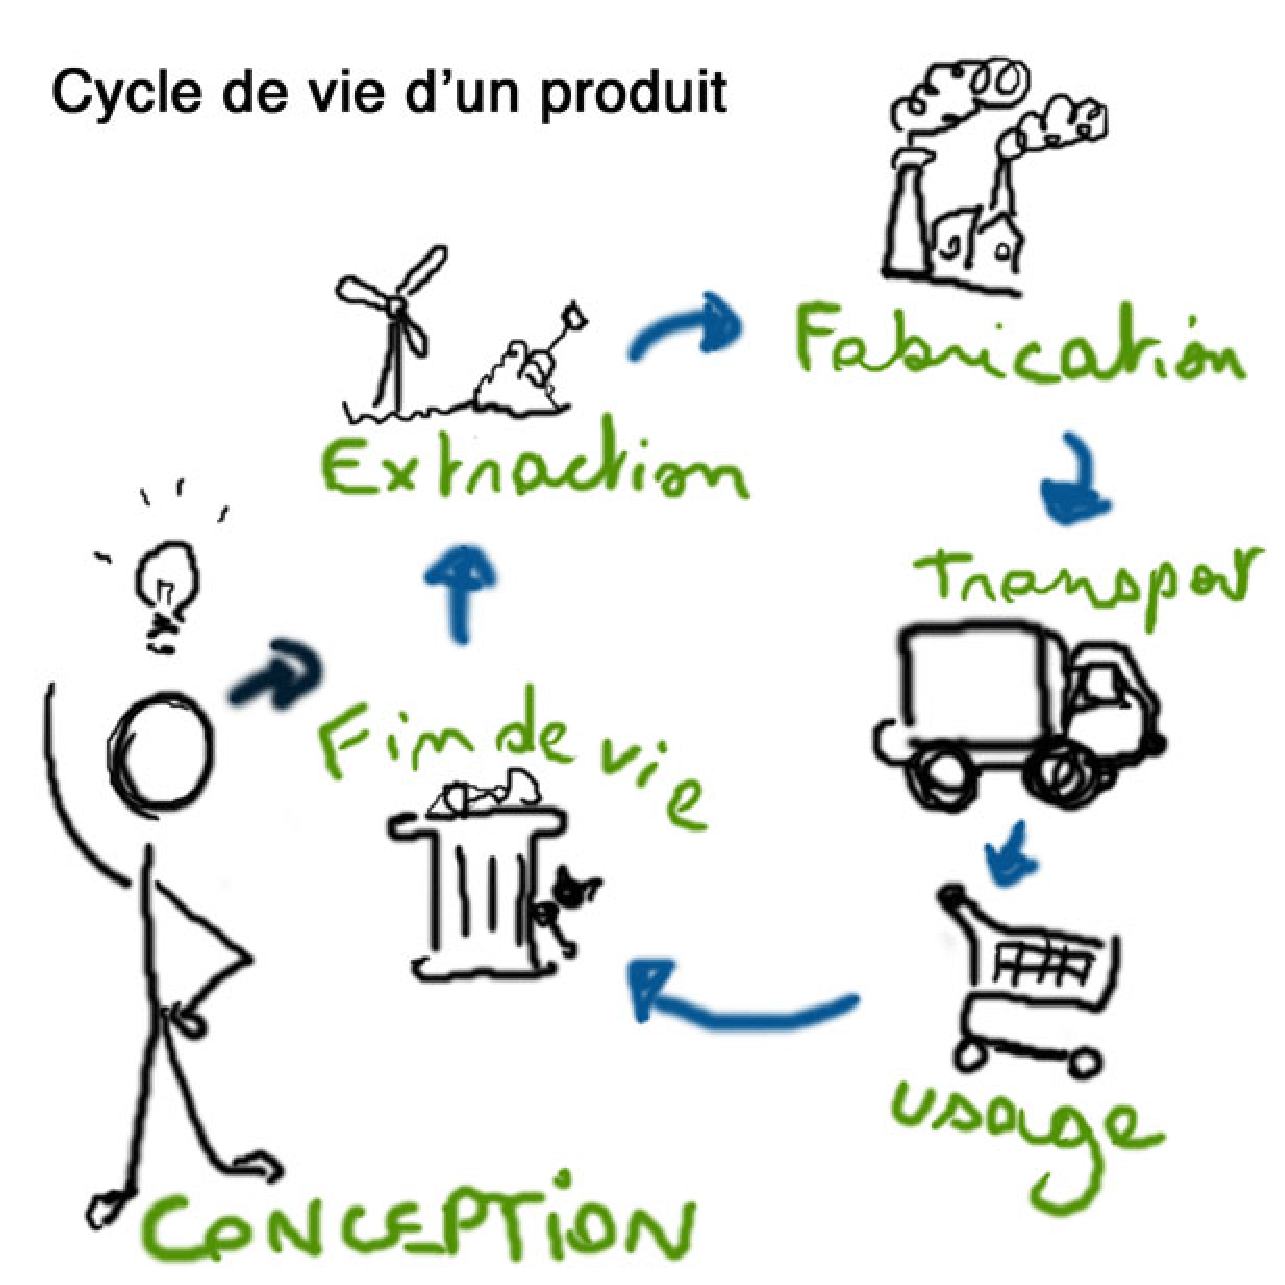
\includegraphics[width=0.6\textwidth]{figures/Cycle-de-vie.eps}
	\caption{Cycle de vie (source : wikipedia, auteur : DamarisBasileJudith)}
	\label{CdV}
\end{figure}

La particularité du produit qu'est le logiciel par rapport aux produits standard de l'industrie (la dématérialisation en particulier) fait qu'il est difficile d'appliquer un modèle existant pour effectier une ACV d'un logiciel. Il serai donc nécéssaire de travailler à l'élaboration d'un modèle propre au logiciel.
			\subsubsection{}
			
		
	\section{La mesure de consommation d'énergie}
	%TODO Finir d'écrire la section sur la mesure de consommation
Dans cet partie de l'état de l'art je vais parler des différentes techniques pour extraire et utiliser une information sur la consommation d'un logiciel.
		\subsection{Différentes approches pour mesurer la consommation des ressources}
			\subsubsection{La mesure par un appareil externe}
La première méthode, la plus commune pour mesurer les resources consommées par un appareil électrique, est de placer un wattmètre en série sur l'alimentation de cet appareil. Avec un wattmètre récent on peut mesurer un ensemble de paramètre tel que les watts, les watts/heure, les volts et les ampères. De plus la plupart des outils récent propose un système d'enregistrement et/ou de transfert des données vers un ordinateur.

\begin{wrapfigure}{dR}{0.3\textwidth}
		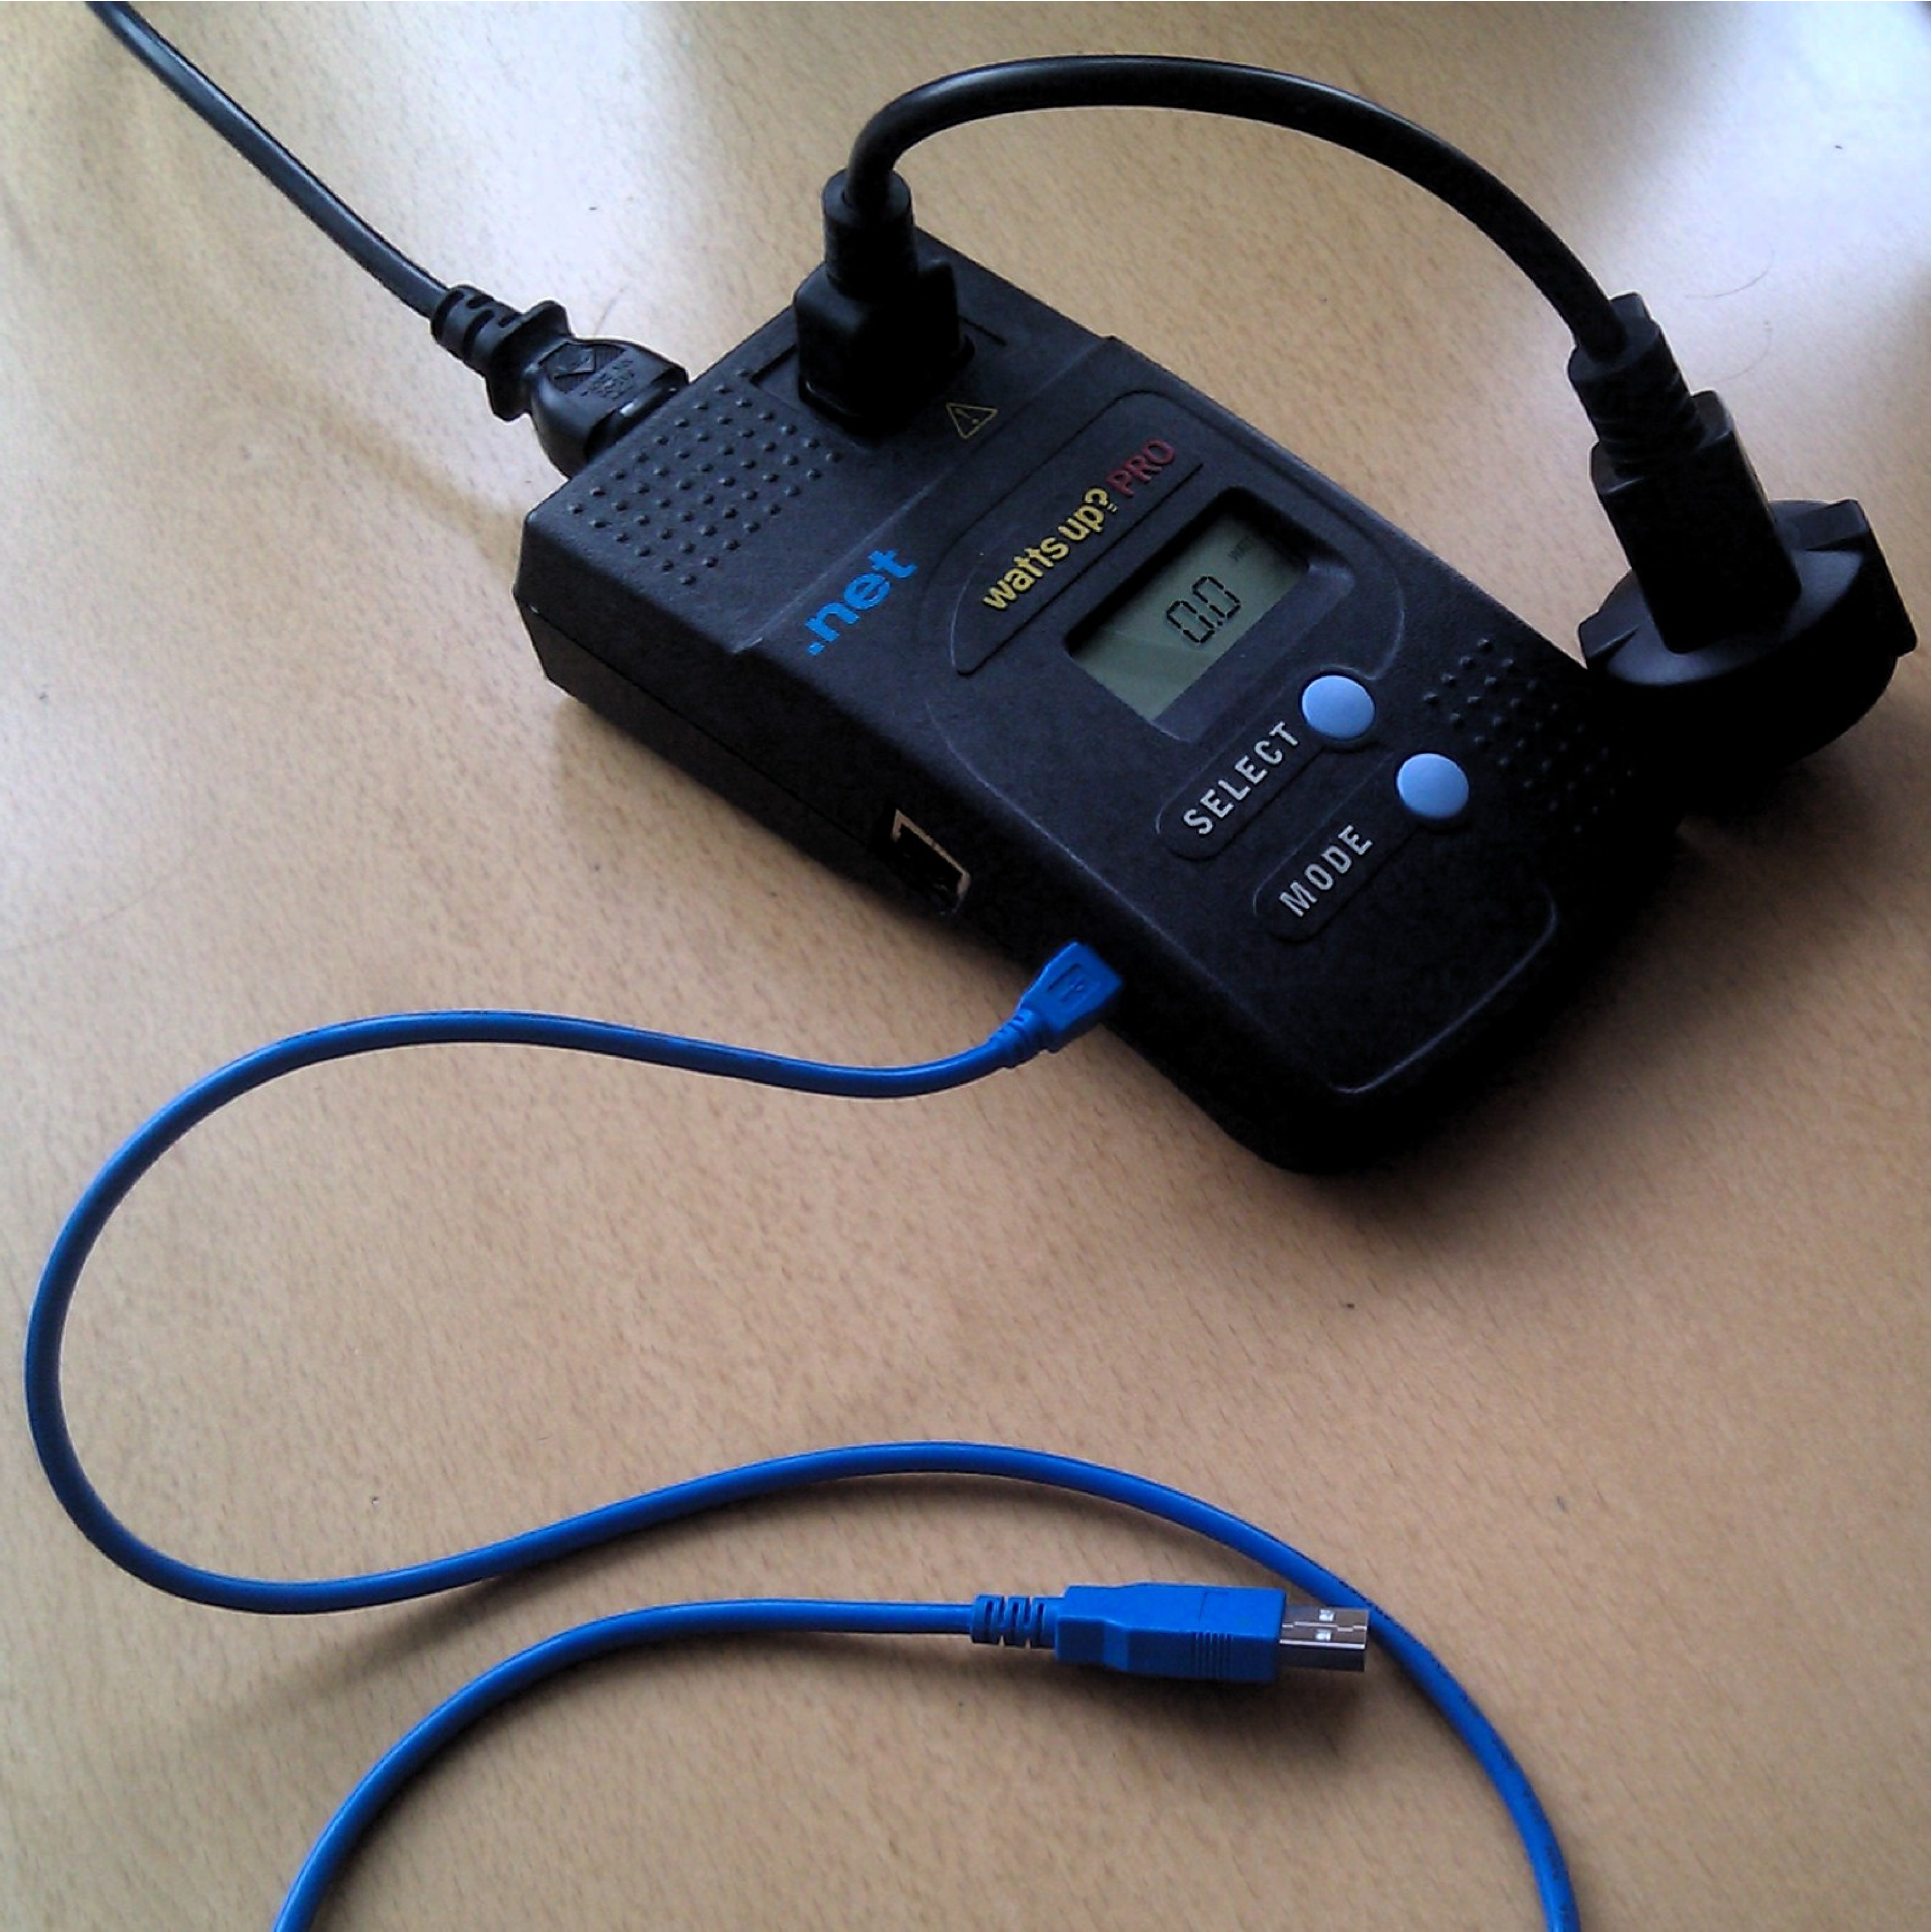
\includegraphics[width=0.3\textwidth]{figures/wattsUp.eps}
		\caption{Photo d'un watts up pro .net}
		\label{wattsUp}
\end{wrapfigure}

Par exemple, les \textit{plugwizes} sont des modules qui se placent sur la prise. sont capable de couper l'alimentation de l'appareil branché dessus et de mesurer la consommation électrique de celui ci. Ils sont capable de transmètre ces informations sans fils jusqu'à un ordinateur. Un autre exemple de ce type de matériel, les wattmètres de la marque \textit{watts up\/?}. Ils permettent, suivant leur gamme, de collecter de l'information et de la transmètre. Le \textit{watts up\/? pro .net} (figure~\ref{wattsUp}) dispose d'un système d'enregitrement de, au maximum, 120000 mesures de watts et de deux interface de communication, USB et Ethernet.

Cette technique de mesure n'offre qu'une vu global de notre système. Il est impossible par cette méthode d'identifier de manière certaine la consommation d'un logiciel. On peut par contre corréler un changement de consommation avec un événement survenu (le démarage d'une application, le lancement d'une tache gourmande en traitement\ldots). 

			\subsubsection{La mesure par un logiciel interne}
La deuxième méthode consiste à analyser les ressources utiliser par un programme et, à partir d'un modèle de consommation, d'en déduire la consommation énergétique de l'application. Différentes ressources peuvent être ciblées. On peut les classer en deux catégories : les unités de calcul (CPU, GPU\ldots) et les dispositifs d'entrées/sorties (disque dur, interface réseau\ldots).

Pour les unités de calcul, deux modèles sont possible pour extraire une consommation. On peut soit utiliser le pourcentage d'utilisation par l'application de l'unité, soit utiliser le temps 

référence à cet article \cite{noureddine:hal-00681560}

			\subsubsection{Vers une mesure par un appareil interne}
Le future !!! des wattmètres/des sondes installer dans chaque composant. référernce à cet article\cite{Esmaeilzadeh:2011:LBL:1950365.1950402}
		
		\subsection{Comment comparer la consommation de deux logiciels}
			\subsubsection{Deux versions d'un logiciel}
Article Green mining\cite{GreenMining} décrivant une méthodologie

			\subsubsection{Deux logiciels isofonctionnel}
Parler des métriques.

			\subsubsection{Deux logiciels diférents}
Parler de métrique plus complexe.
		
	\section{Fabriquer un éco-logiciel}
	%TODO Ecrire la section Fabriquer un eco-logiciel
		\subsection{De la Conception\ldots}
		
		\subsection{\ldots~À la programmation}
		
		\subsection{La programmation Modulaire}
			\subsubsection{Intéret de la programmation modulaire dans l'économie d'énergie}
			\subsubsection{OSGi : du java modulaire}
		
		
		
	\section{Travaux similaire}
	%TODO Ecrire la section Travaux similaire
Dans cette section je vais présenter les projets en rapport avec mon sujet de stage et dont j'ai soit entendu parler soit pu rencontrer les acteurs.
		\subsection{Le Green code Lab}
Le green code lab est un groupement de personne souhaitant promouvoir le développement durable dans le logiciel. C'est une communauté virtuelle qui se charge de publié des articles d'informations, d'organiser des évenements et des formation autour de l'éco-conception de logiciel.

Leur site internet (\href{http://www.greencodelab.fr}{www.greencodelab.fr}) sert de plateforme de publication de leurs article. Ils ont aussi mit en place un GitHub qui sert de laboratoire pour effectuer des expérimentations. Enfin le green code lab a publié un livre intitulé \textit{Green Pattern - Manuel d'éco-conception des logiciels} et disponible à la vente au format papier ou numérique.

Durant mon stage, j'ai eu l'occasion de me rendre à l'un de leurs évenements sur le thème de la mesure de la consommation électrique d'un logiciel. Là bas, Olivier Philippot, un membre actif du green code lab, nous à présenté une méthodologie basé sur des \textit{plugwizes} en affichant les mesure au moyen du logiciel KST.
		\subsection{Le projet code vert}

		
	\section{Conclusion}
	%TODO Ecrire la section Conclusion de l'état de l'art

\chapter{Comment peut on mesurer la consommation d'un logiciel ?}
%TODO écrire le chapitre Comment peut on mesurer la consommation d'un logiciel
	\section{Qu'est ce qui consomme dans un ordinateur ?}
	\section{Outils de mesure de la consommation des ressources par un logiciel}
		\subsection{Ptop}
pTop est un programme de collecte d’information sur l'exécution de processus sous linux. Il est censé récupérer les données sur l'utilisation du CPU, de la RAM et des échange réseaux. Il doit ensuite être capable, une fois le modèle paramétré, sortir des informations sur la consommation énergétique.

Malheureusement, il s'est avéré que pTop ne fonctionne pas entièrement. Après plusieurs essais infructueux, j'ai supposé que le logiciel avait été abandonné sans être fini.

			\subsubsection{Procédure d'installation}
\begin{itemize}
    \item récupérer les sources sur http://mist.cs.wayne.edu/ptop.html
    \item installation du nécessaire pour compiler les sources (paquets debian) :
    \begin{itemize}
	\item build-essential
	\item libmysqlclient-dev
	\item libncurses-dev
    \end{itemize}
    \item Installation de la base de données Mysql :
    \begin{itemize}
	\item création d’une base de donées ptop
	\item exécution du script db\_schema.sql
	\item remplacement du login et password pour accéder à la base de données dans le fichier database.c
    \end{itemize}
    \item Compilation :
\end{itemize}

\begin{verbatim}
	# make
	# chmod +x ptop
\end{verbatim}

\subsubsection{Exécution}
Lancer le programme au moyen de la commande :

\begin{verbatim}
# ./ptop
\end{verbatim}

Le programme va s'initialiser et enregistrer les mesures dans les bases de données. Il faut ensuite interrompre les mesures au moyen du signal SIGINT.

\subsubsection{Données de sortie}
Il n’existe pas, à ma connaissance, de documentation précise sur les données de sortie du programme pTop.  Le programme stock les données dans une base de données Mysql nommé ptop. Elle est composée de quatre tables :
\begin{itemize}
	\item device\_energy
	\item process\_energy
	\item process\_info
	\item sys\_info
\end{itemize}

Seul les deux dernières tables sont remplies par le programme (à cause soit d’un bug, soit d’une version non finit du programme).

\subsection{Energy Checker}
Le projet Energy Checker développé par Intel, est un ensemble d’outil destiné à faciliter la remontée et l’affichage des mesures faites sur la consommation d’un programme. Il se compose principalement de l’API energy checker qui permet d’utiliser les mécanismes de remonter d’information (PL - Productivity Link)

\subsection{ClassMexer}
ClassMexer est un API java permettant d’estimer la taille en mémoire d’un objet java. On peut télécharger cet API sous la forme d’un fichier JAR à cette adresse : http://www.javamex.com/classmexer/. ClassMexer est un Instrumentation agent comme spécifié dans le pattern Instrument. Cela implique de travailler avec, au minimum, la version 5 de java.

\subsubsection{procédure d'installation}
\begin{itemize}
	\item Télécharger l’API
	\item Importer le fichier JAR dans le projet.
	\item Insérer des appels sur l’objet que l’on souhaite mesurer. Par exemple :
\begin{verbatim}
public class Main {
	public static void main(String[] args) {
		String str = "Hello world !";
		
		long noBytes = MemoryUtil.deepMemoryUsageOf(str);
		
		System.out.println(noBytes);
	}
}
\end{verbatim}
	\item Exécuter le programme avec l’option -javaagent:<fichier JAR>
\end{itemize}

\subsection{JouleMeter}
Joulemeter est un outil développé par Microsoft et qui sert à mesurer la consommation d’énergie sur un ordinateur. Il ne fonctionne que sous Windows 7.

\subsubsection{Procédure d'installation}
\begin{itemize}
	\item Télécharger le logiciel sur ce site : Joulemeter
	\item Exécuter le programme.
\end{itemize}

\subsubsection{Fonctionnement}
Joulemeter est un logiciel de mesure qui se base sur un modèle de consommation. La première étape est donc de générer ce modèle. Deux méthodes existent.

La première n’est utilisable que sur un ordinateur portable muni d’une batterie. Il suffit de débrancher l’alimentation et de lancer la calibration (15 minuntes sans utiliser le PC). Avant de lancer la calibration, il faut faire attention à arrêter toutes les application afin que le logiciel puisse déterminer une consommation minimum en mode "Idle".

Le deuxième mode nécessite un Wattmètre WattsUp pour générer le modèle. Il suffit de le brancher en USB, de couper toutes les applications possible et de lancer la calibration (3 minutes sans utiliser le PC).

\subsection{PowerAPI}
PowerAPI est un outil sur lequel travail l'équipe ADAM de l'université de Lille. Les premiers résultats de cet outil ont été présentés dans un papier\cite{noureddine:hal-00681560} publié à l'ICSE\footnote{International Conference on Software Engineering} 2012 à Zurich. Cet outil parait prommetteur et s'il continu à être développé, pourait bien apporter une solution intéressante au problème de la mesure de consommation énergétique de logiciel.

Selon la présentation qui en a été faite, il fonctionne actuellement pour la consommation CPU. Cet outil collecte le temps CPU d'un processus et la fréquence de celui-ci en temps réel. Puis il détermine l'énergie consommée grâce à des tables de consommations par rapport à la fréquence fournis par les fabriquant de processeur.

Je n'ai malheureusement pas essayé PowerAPI par manque de temps. Je n'ai eu accès au programme que tardivement durant mon stage et à ce moment je travaillais sur d'autres aspects.

\chapter{Mise en valeur de l'impact du code sur la consommation}
%TODO écrire le chapitre Mise en valeur de l'impact du code sur la consommation
Tout au long de mon stage j'ai développé un ensemble de petits programmes qui mettent en valeur une bonne pratique à adopter, la faiblesse d'un mécanisme ou encore l'importances des choix effectué durant le développement d'un logiciel. Dans ce chapitre je vais présenter les exemples les plus éloquants. 
	\section{Impact du choix du langage}
	\section{Impact des choix de programmation}
		\subsection{Description des tests}
		\subsection{Resultats obtenus}

\chapter{La programmation modulaire au service de l'économie d'énergie}
%TODO écrire le chapitre La programmation modulaire au service de l'économie d'énergie
Afin de mettre en valeur l'importance de l'architecture logiciel dans la consommation, j'ai proposé de développer une application basé sur la technologie java OSGi\footnote{\href{http://www.osgi.org}{www.osgi.org}}. L'objectif de ce projet est de pouvoir réaliser facilement des démonstrations d'application modulaire qui s'adapte en fonction de contrainte énergétique. J'ai donc choisi d'élaborer un quadriciel qui permettrai d'échanger une partie de l'application (dans notre context un bundle OSGi) contre une autre afin d'optimiser la consommation. Afin d'expliquer plus clairement le but du projet, je vais détailler un cas d'utilisation du cadriciel.

Un programme doit réaliser une tache. Le développeur connait deux algorithmes pour coder cette tache. Ils ont chacun leurs forces et leurs faiblesses. La version A du code consomme peu d'énergie en temps normale (figure~\ref{AbsBdlA}). Mais, dans certaines condition, ici quand un évenement A se produit, l'algorithme se met à surconsommer. La version B du code, elle, consomme plus d'énergie (figure~\ref{AbsBdlB}) que la version A. Par contre il est moins sensible à l'arriver de l'évenement A. Donc pour réaliser cette tache en économisant le plus d'énergie il faudrait exécuter le code A en temps normal, et le code B quand l'évenement A se produit. La solution de mettre les deux algorithmes dans le même programme n'est pas une bonne solution. En faisant de la sorte, on alourdit le programme, ce qui rend plus exigent en ressource le programme et donc avance l'obsolescence des machine. De plus, cela rend la maintenance du code plus difficile.


\begin{figure}
        \begin{subfigure}[b]{0.45\textwidth}
                \centering
                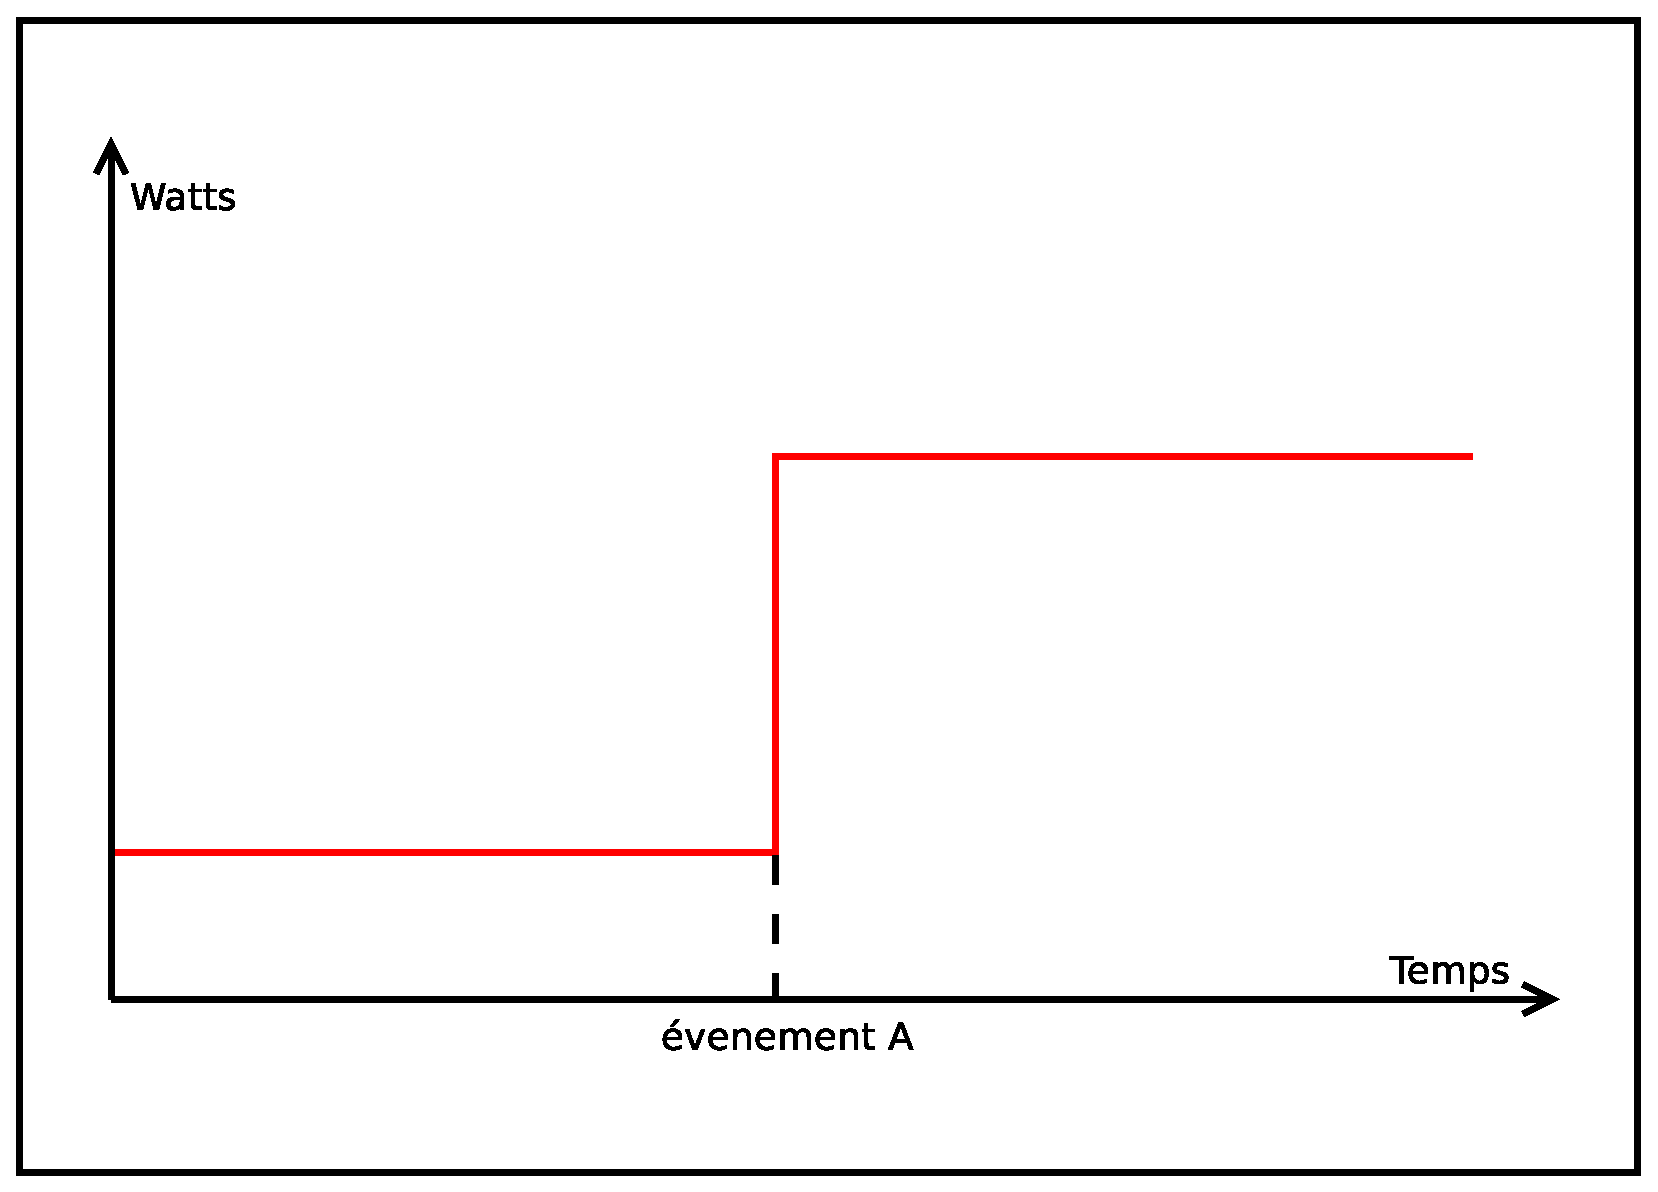
\includegraphics[width=\textwidth]{figures/Abstract_bundle_A.eps}
                \caption{Consommation du bundle A}
                \label{AbsBdlA}
        \end{subfigure}
        ~
        \begin{subfigure}[b]{0.45\textwidth}
                \centering
                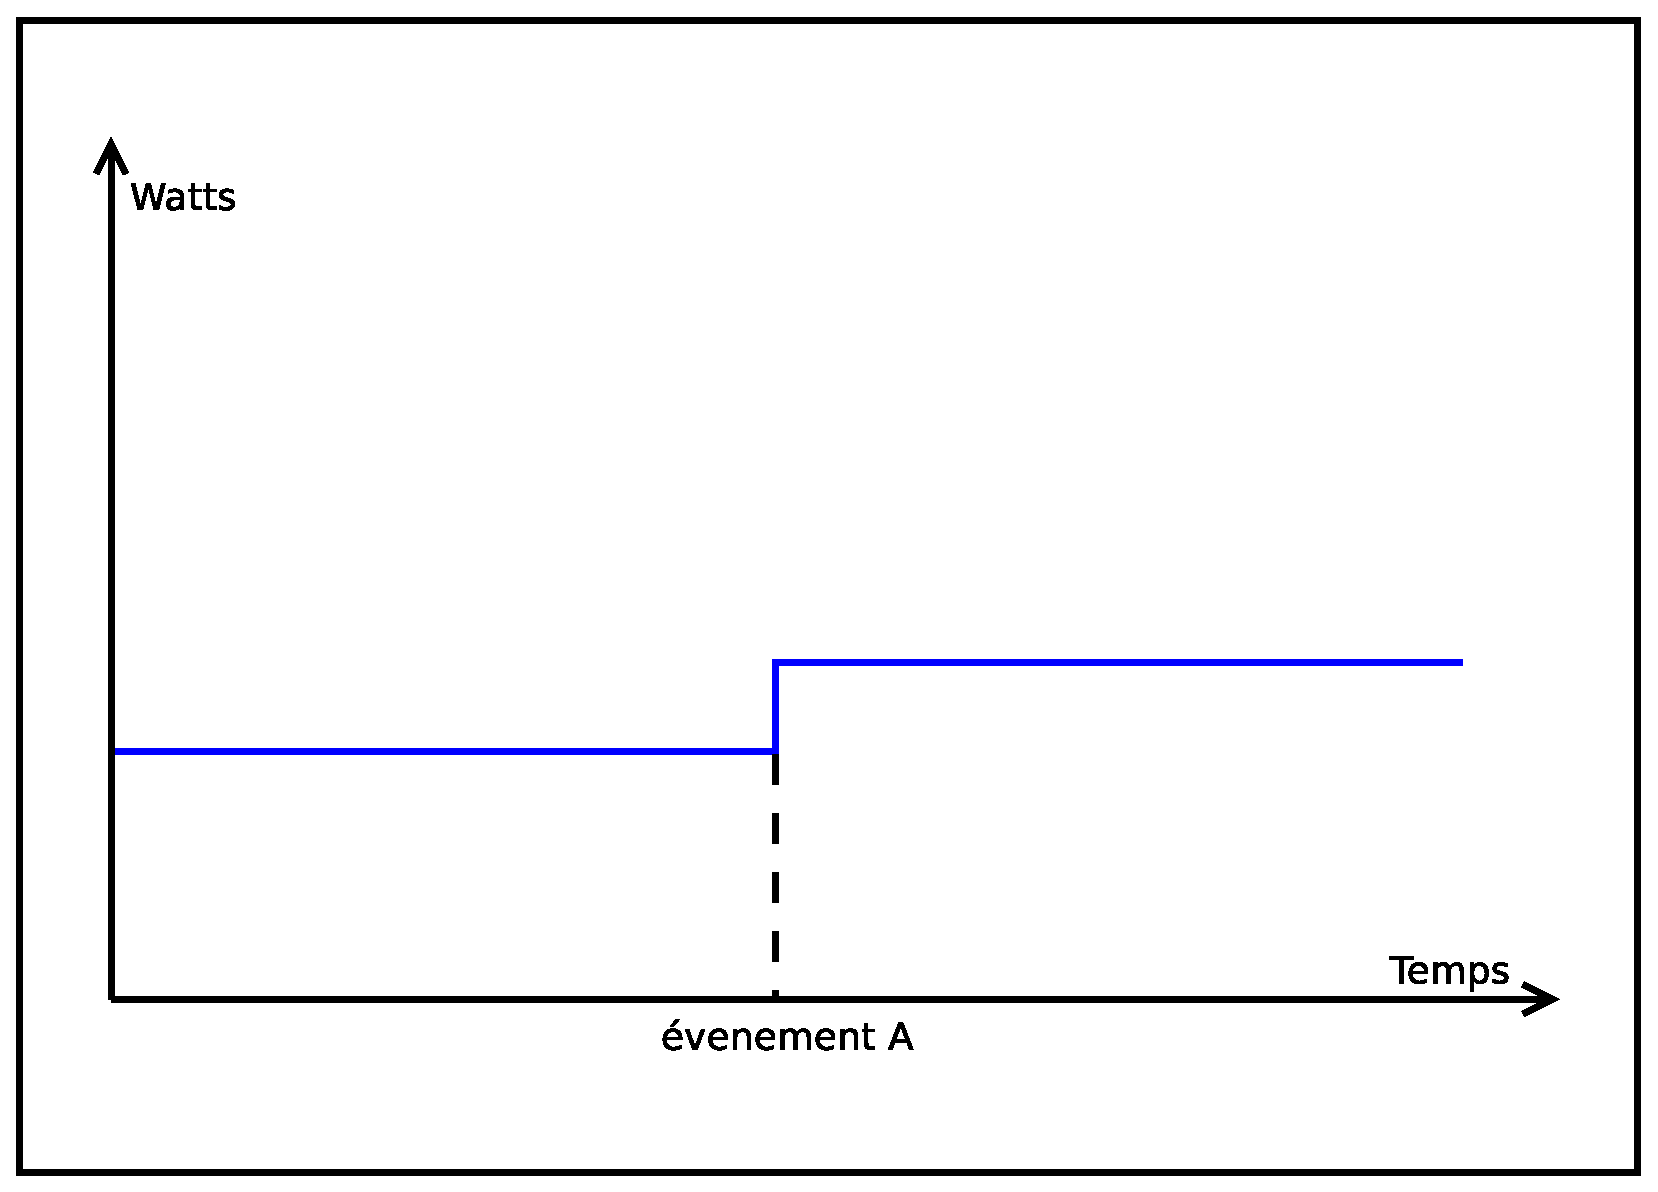
\includegraphics[width=\textwidth]{figures/Abstract_bundle_B.eps}
                \caption{Consommation du bundle B}
                \label{AbsBdlB}
        \end{subfigure}
        \caption{Illustration de l’optimisation de la consommation par l’échange de bundle}
        \label{AbsBdl}
\end{figure}

Le cadriciel que j'ai dévellopé a pour but de remplacer à chaud le code de le code A contenu dans un \textit{bundle OSGi} par le code B contenu dans un autre \textit{bundle} lorsqu'il est interressant de le faire. Il y a d'autre cas d'utilisation que l'on pourrait imaginer tel que la mise en place d'une politique énergétique sur une machine (par exemple réduire la consommation d'une machine utilisant l'énergie solaire pendant la nuit).

	\section{Présentation de l'infrastructure développé}
Cette infrastructure est entièrement basé sur OSGi. Elle a donc été conçu sous la forme de modules indépendants les uns des autres. On peut voir sur la figure~\ref{BdlDiag} les modules ainsi que les liaisons entre ces modules. Une flèche d'un module A vers un module B signifie que le module A à besoin de B pour pouvoir fonctionner. Dans cet section je vais détailler l'utilité, voir le fonctionnement de chacun des modules.
	
\begin{figure}
	\centering
	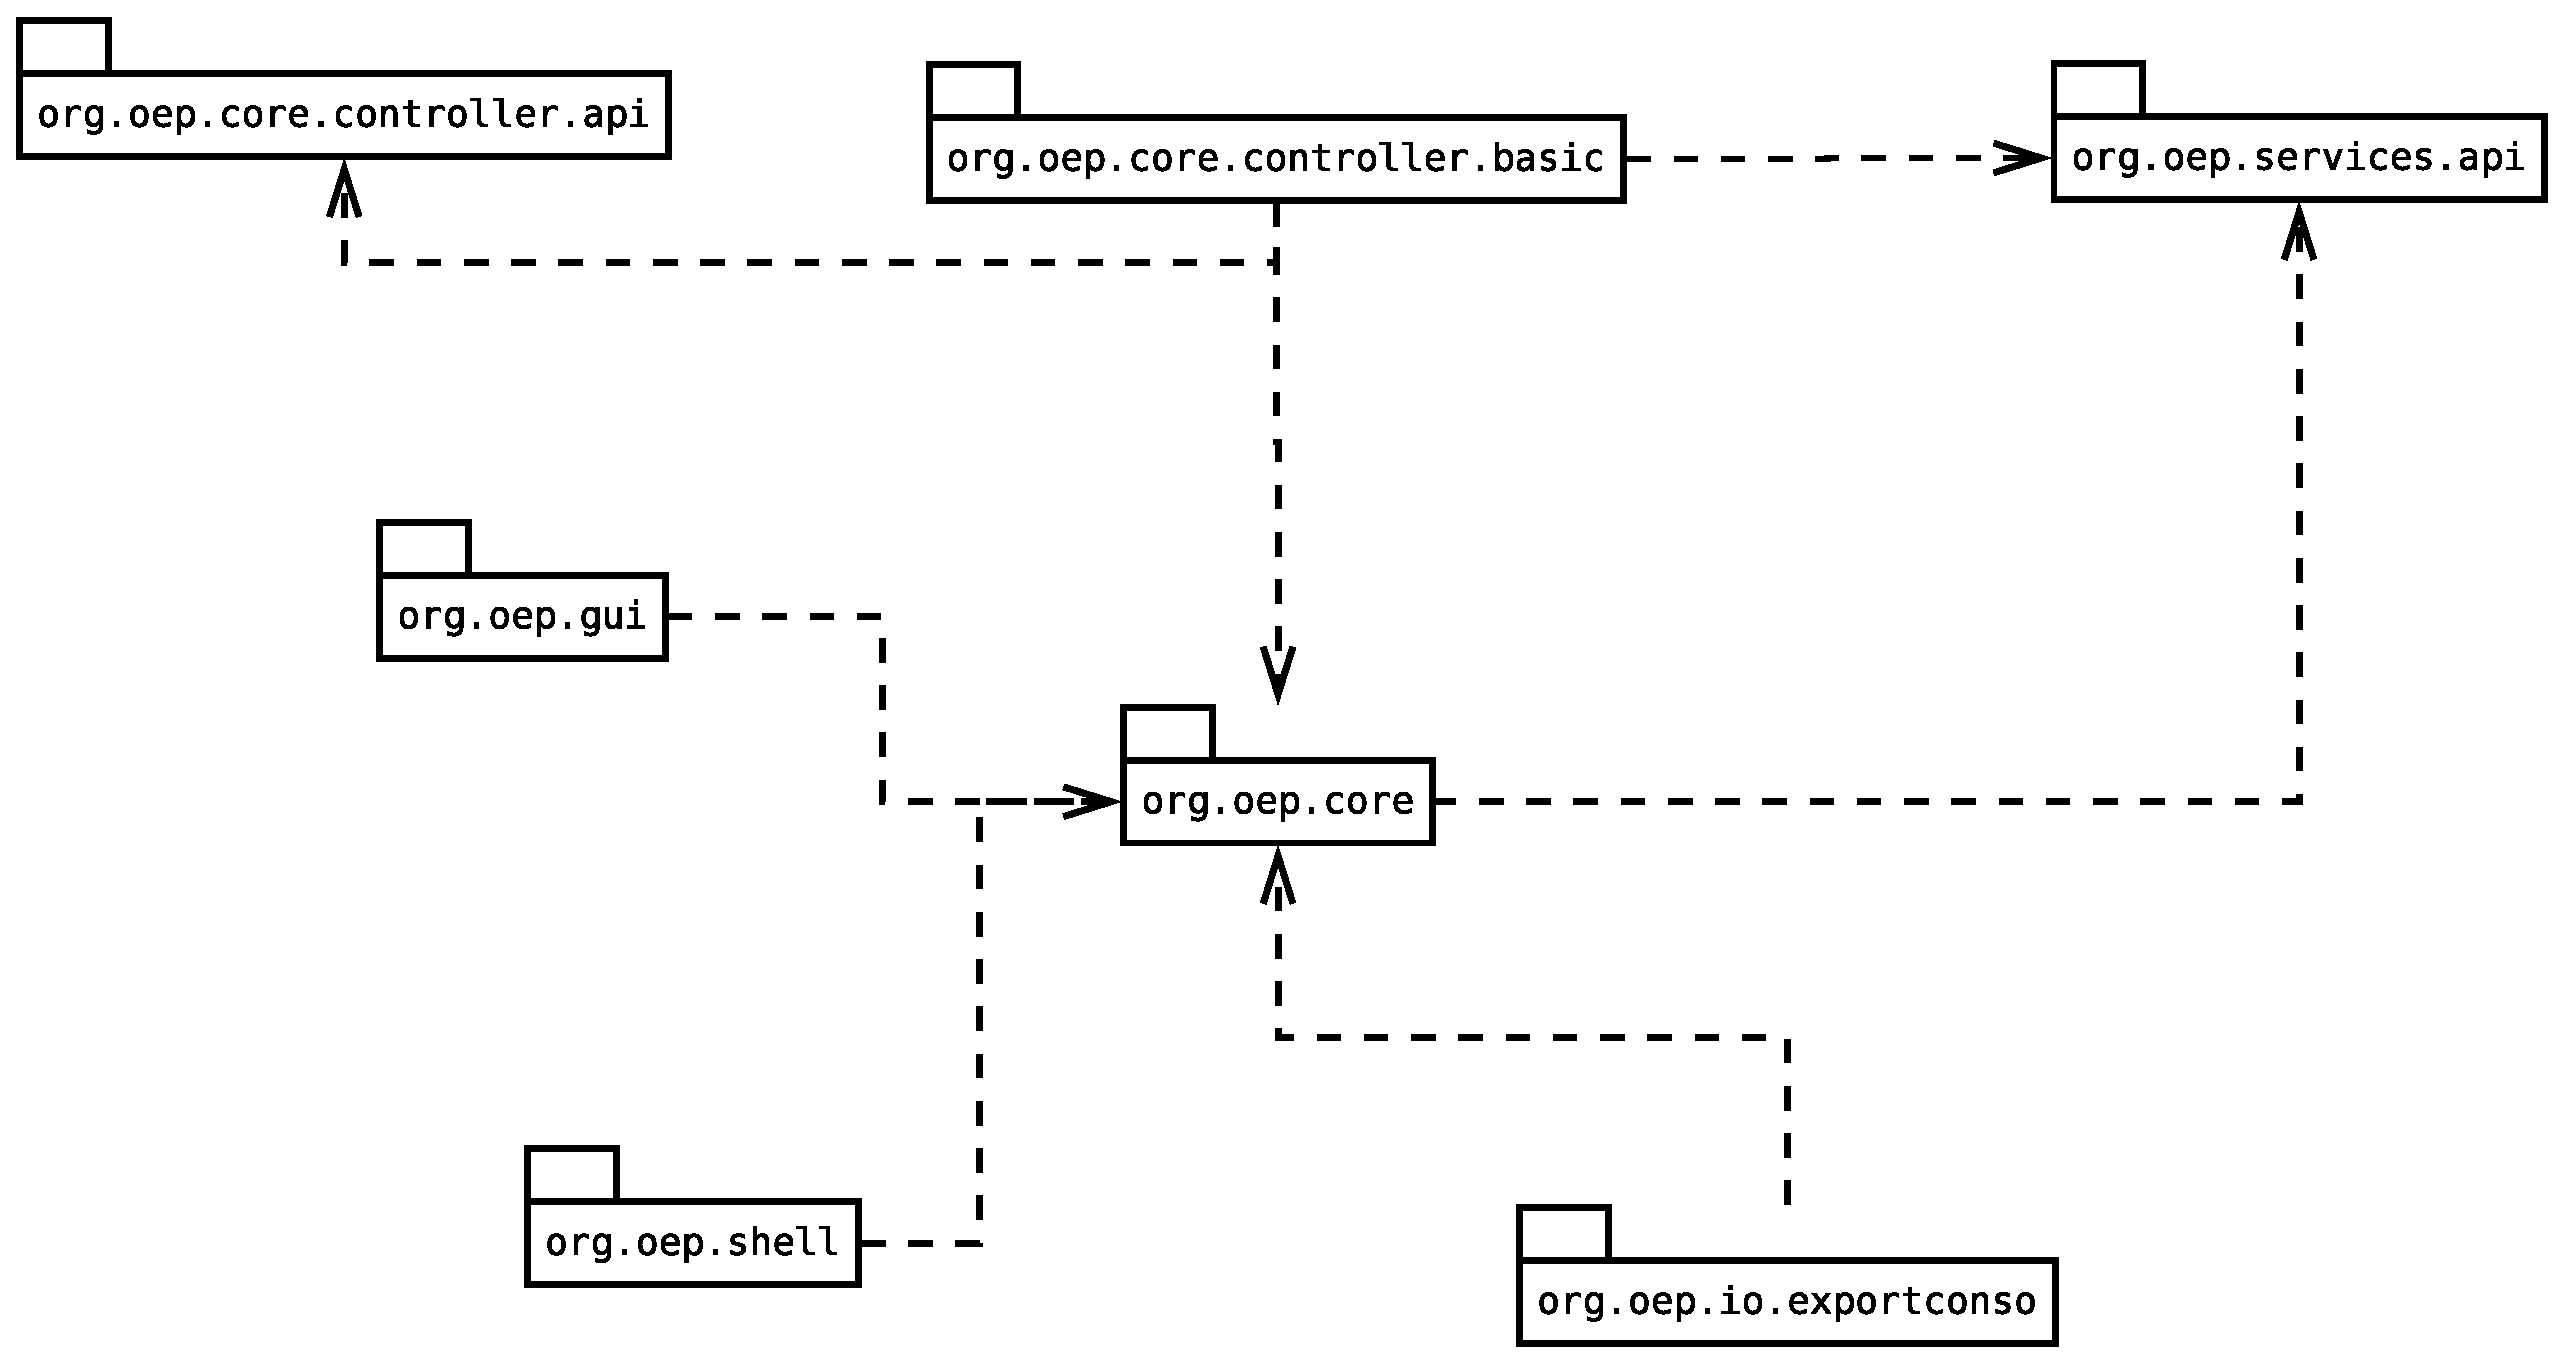
\includegraphics[width=0.95\textwidth]{figures/EcoPattern_Bundle_Diagramme.eps}
	\caption{OSGiEcoFramework : diagramme de liaison des bundles}
	\label{BdlDiag}
\end{figure}
\subsection{Le coeur du système}
La partie central du cadriciel se trouve dans le package \textit{org.oep.core}. Il se découpe en deux classes qui gèrent l'application que l'on souhaite faire fonctionner. La première est la classe \textit{BundleManager}. C'est elle qui s'occupe de gérer les modules qui forment l'application. Elle permet d'installer deux types de modules. Ceux définnissant un service et ceux rendant un service. C'est ensuite par cette classe que l'on démarre ou arrête un module offrant un service. Le \textit{BundleManager} garantit qu'il n'y ai qu'un et un seul module démaré par service.

La deuxième classe, \textit{ServiceManager}, s'occupe de référencer les services démarrés. Pour cela elle implémente l'interface \textit{ServiceListener}. Elle permet ensuite de consulter leur consomation au travers de l'inter1face \textit{EcoService}.
		\subsection{Les interfaces}
J'ai développé deux types d'interfaces pour ce framework. Une première graphique, basé sur la technologie \textit{Swing}, l'autre en ligne de commande. L'interface graphique est découpé en deux vues. Une pour installer des services (figure~\ref{BdlList}) et l'autre pour démarrer ou arrêter les services ainsi qu'afficher la consommation (figure~\ref{RngList}).

\begin{figure}
	\centering
	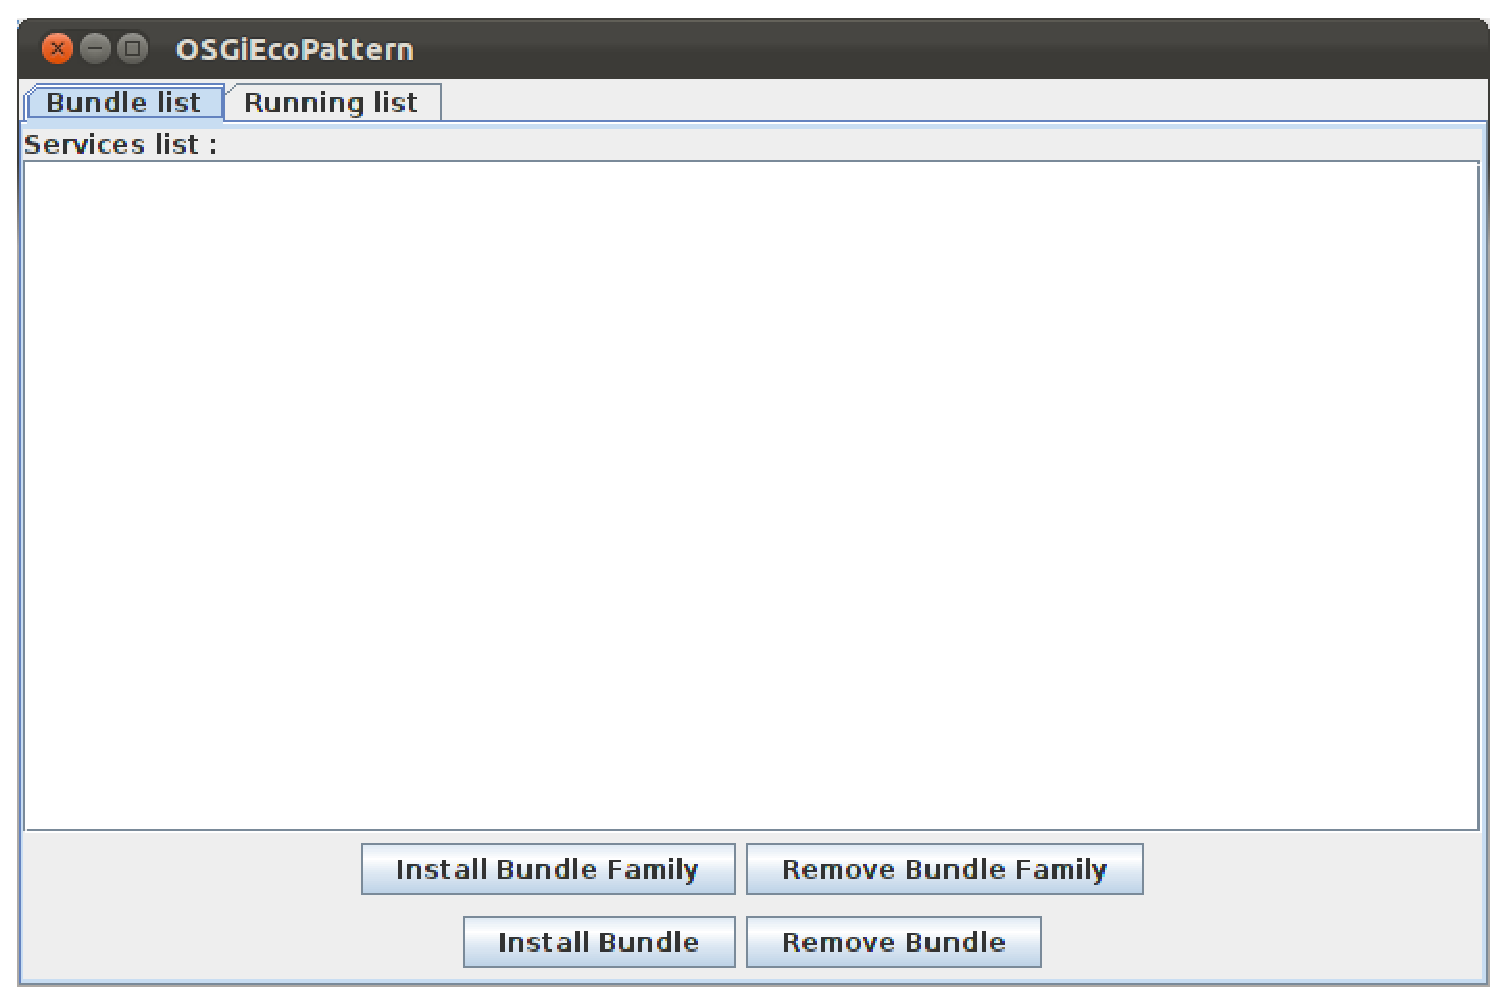
\includegraphics[width=0.95\textwidth]{figures/EcoPattern_Bundle_List_View.eps}
	\caption{Interface d'instalation des services}
	\label{BdlList}
\end{figure}
\begin{figure}
	\centering
	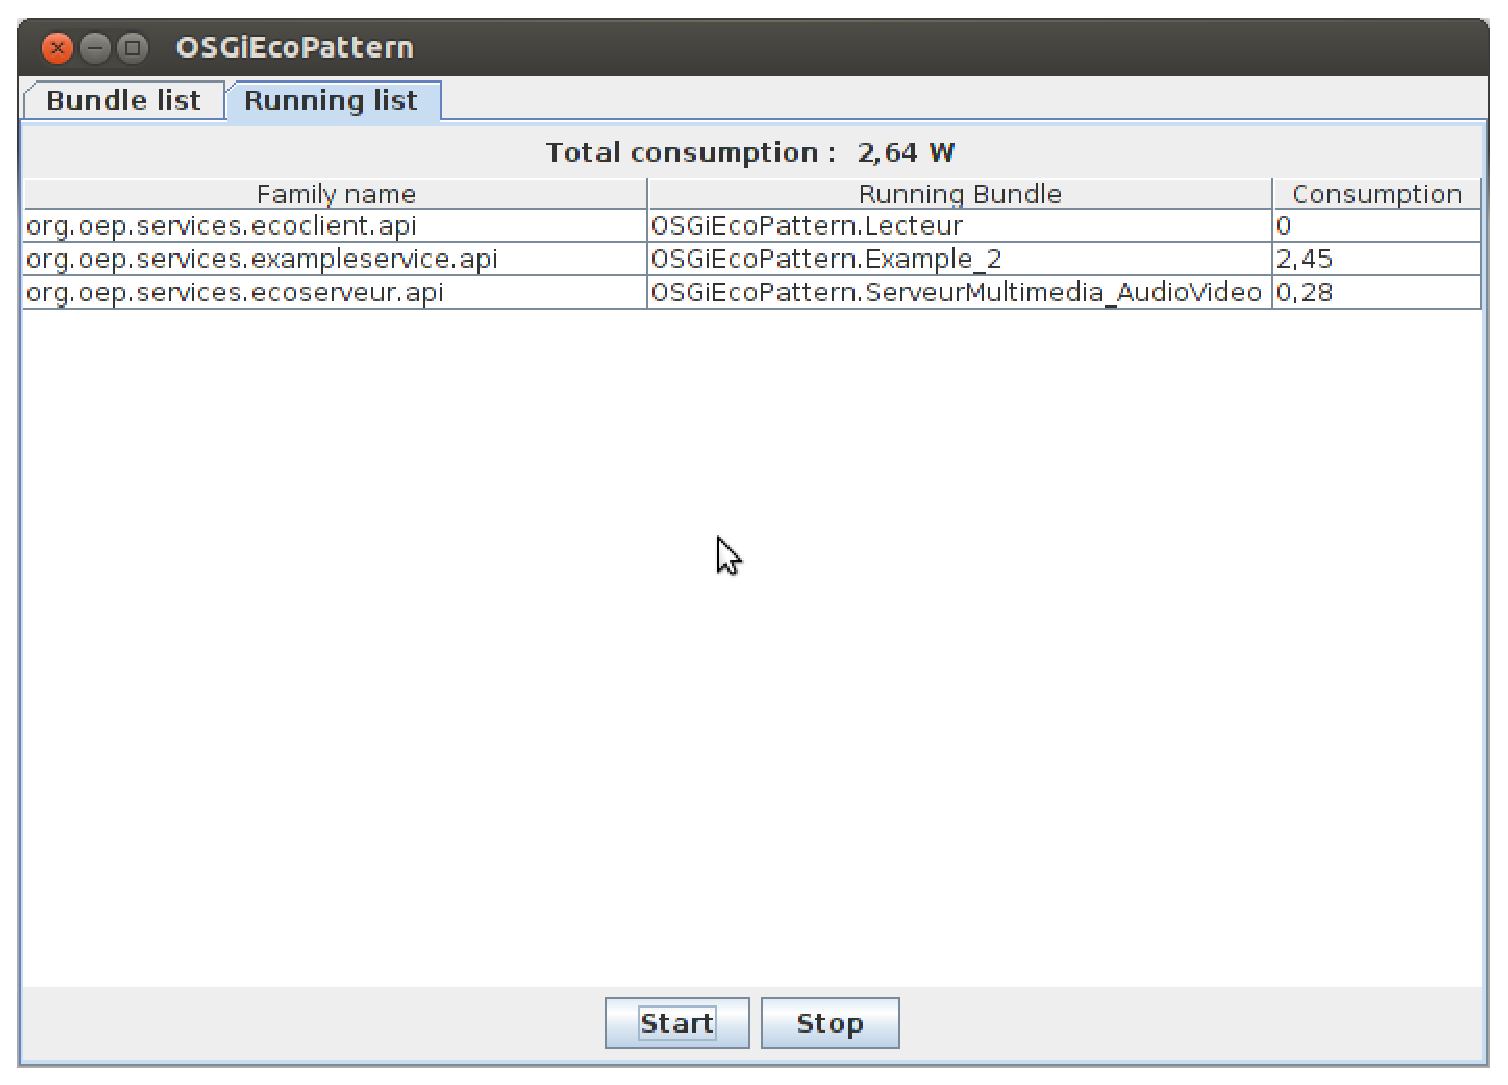
\includegraphics[width=0.95\textwidth]{figures/EcoPattern_Running_List_View.eps}
	\caption{Interface de gestion des services démarés}
	\label{RngList}
\end{figure}

L'interface en ligne de commande est basé sur le shell felix\footnote{http://felix.apache.org/site/apache-felix-shell.html}. j'ai définis seulemment trois commande :
\begin{itemize}
  \item une pour installer une famille de module
  \item une pour installer un module
  \item une pour obtenir la consommation global
\end{itemize}
Pour obtenir un shell complet, il faudrait ajouter à cela une commande pour démarer, une commande pour arrêter et une commande pour obtenir la consommation d'un bundle. Je n'ai pas écris ces commandes car j'ai choisi de privilégier l'interface graphique qui me paraissait plus pertinente pour faire des démonstration.

En plus des interface utilisatrice, j'ai conçu un bundle qui s'occupe d'exporter les données de consommation vers un fichier \textit{CSV}. Cela permet de faire facilement des sauvegarde d'historique de consommation ou bien d'afficher en temps réél une courbe au moyen du logiciel KST.
 
		\subsection{Le controlleur}
Le controlleur est la partie sur laquelle j'ai pu le moins travailler. Il est charger de détecter des changement dans la consommation des modules et de déclancher une action de reconfiguration si besoin. Je souhaitais utiliser pour cela l'API \textit{Wildcat}\footnote{http://wildcat.ow2.org/}. C'est un projet de l'OW2 consortum qui a pour but de fournir un cadriciel permettant la mise en place de sondes et de déclancher des évenements au moyen de requêtes écrite dans un langage proche du SQL.

J'ai abandoné cette solution après avoir passé plusieurs jour à tenter d'intégrer wildcat dans un module OSGi sans y arriver (ceci  à cause de problème de dépendance à d'autre bibliothèque). J'ai donc finalement opté (un peu dans l'urgence) pour une solution plus basique qui vient tester tour à tour chaque bundle pour vérifier qu'il ne dépasse pas une limite de consommation. Cette version du controlleur ne permet pas de mettre en place une politique de consommation élaboré, mais cela m'a permis de faire fonctionner le cadriciel dans le temps imparti pour mon stage. Étant donné qu'il est totaltement indépendant de du reste du cadriciel, on peut facilement le remplacer par un autre plus complexe.
   
		\subsection{Les Services}
 
	\section{Développer une application pour ce framework}

	
	\section{Un exemple d'application : lecteur audio}
Afin d'illustrer les possibilités de ce framework, j'ai développé un exemple concret d'application. Cette application est un simple lecteur multimedia. Sa particularité est que quand on a besoin d'économiser l'énergie il n'affiche plus l'image et ne diffuse que le son de fichier numérique.

\chapter{Conclusion}
%TODO écrire la conclusion.

\bibliographystyle{plain}
\bibliography{biblio}
\listoffigures{}
\listoftables{}
\appendix

\chapter{Sujet de stage}
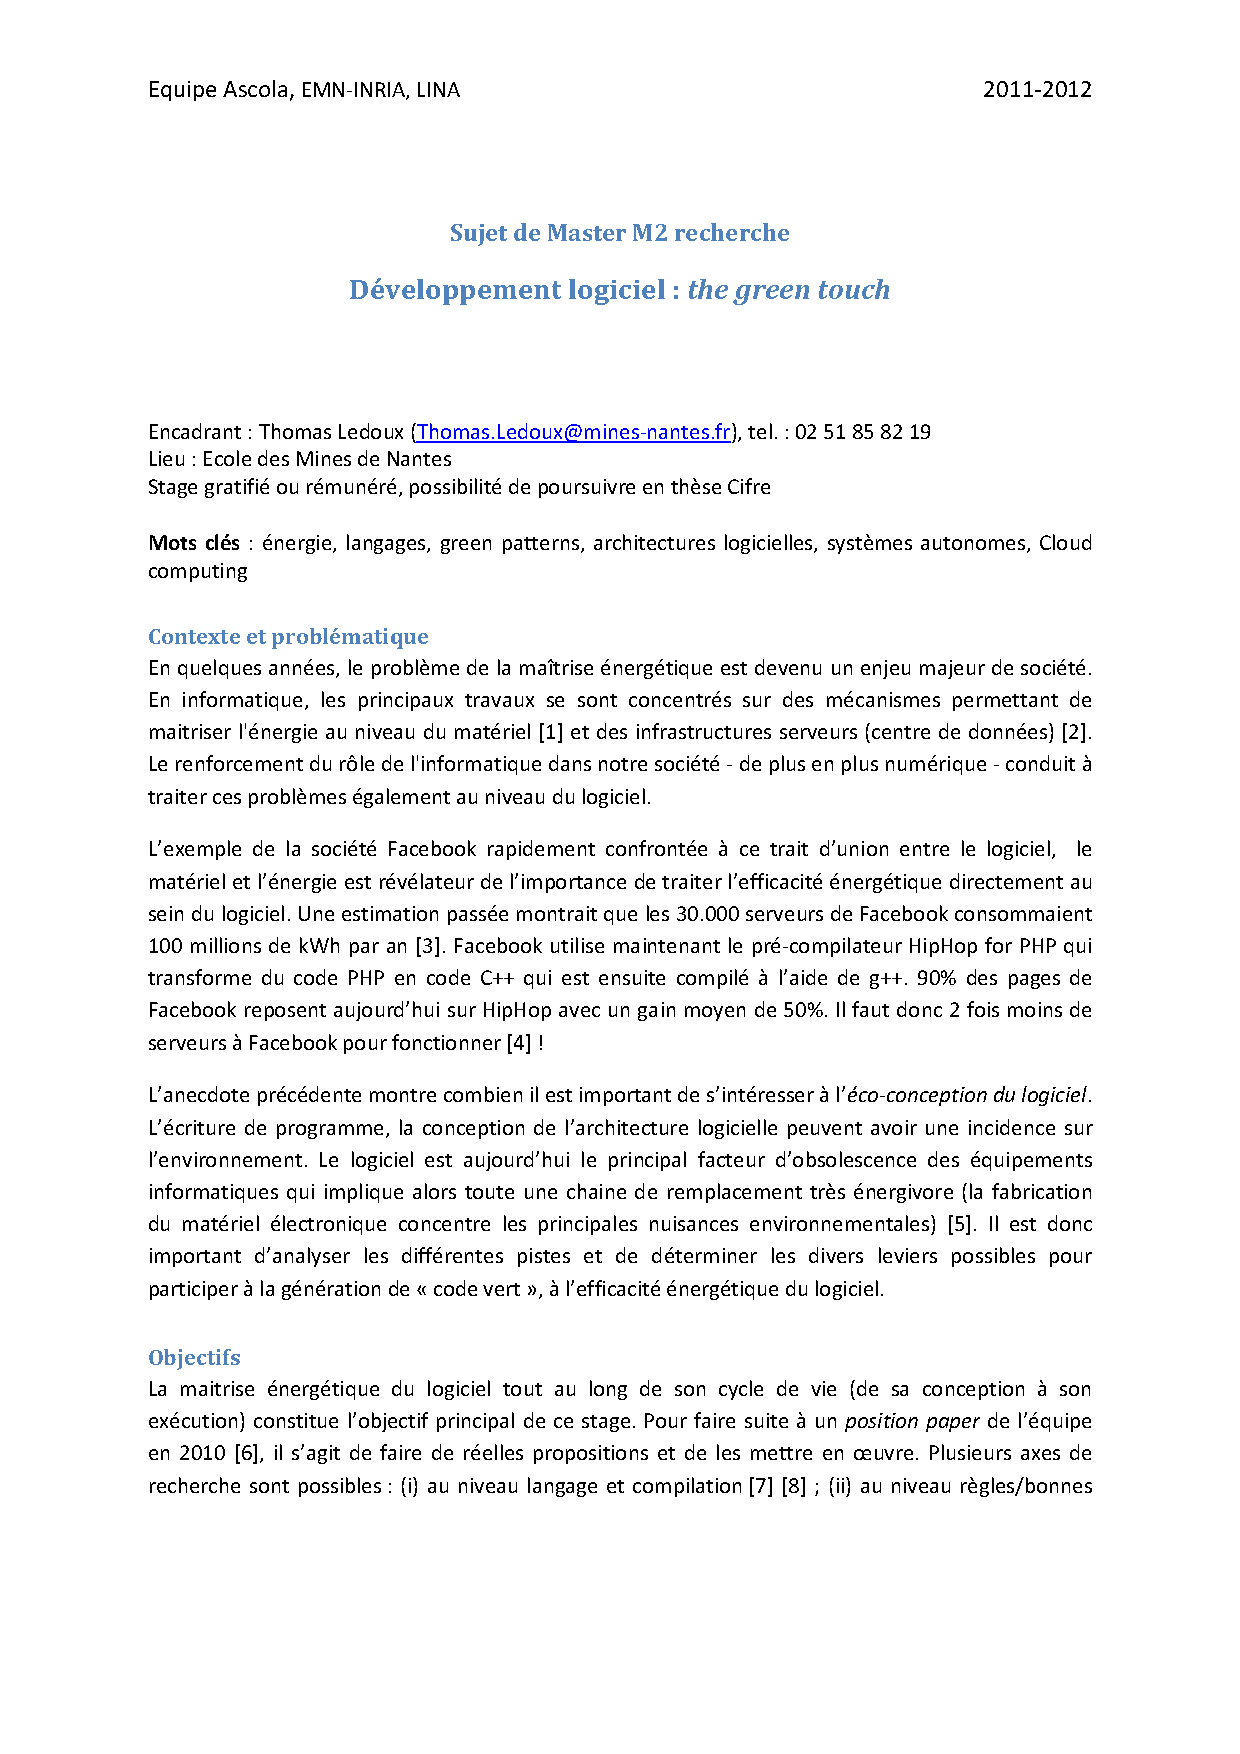
\includepdf[lastpage=3;pages=-]{imports/Sujet_Master_EcoConceptionGL.pdf}

\chapter{Plannification}
%TODO insérer le diagramme de GANT

\chapter{Diagrammes de Classes d'EcoFramework}
\section{Package org.oep.core}
	\begin{centering}
		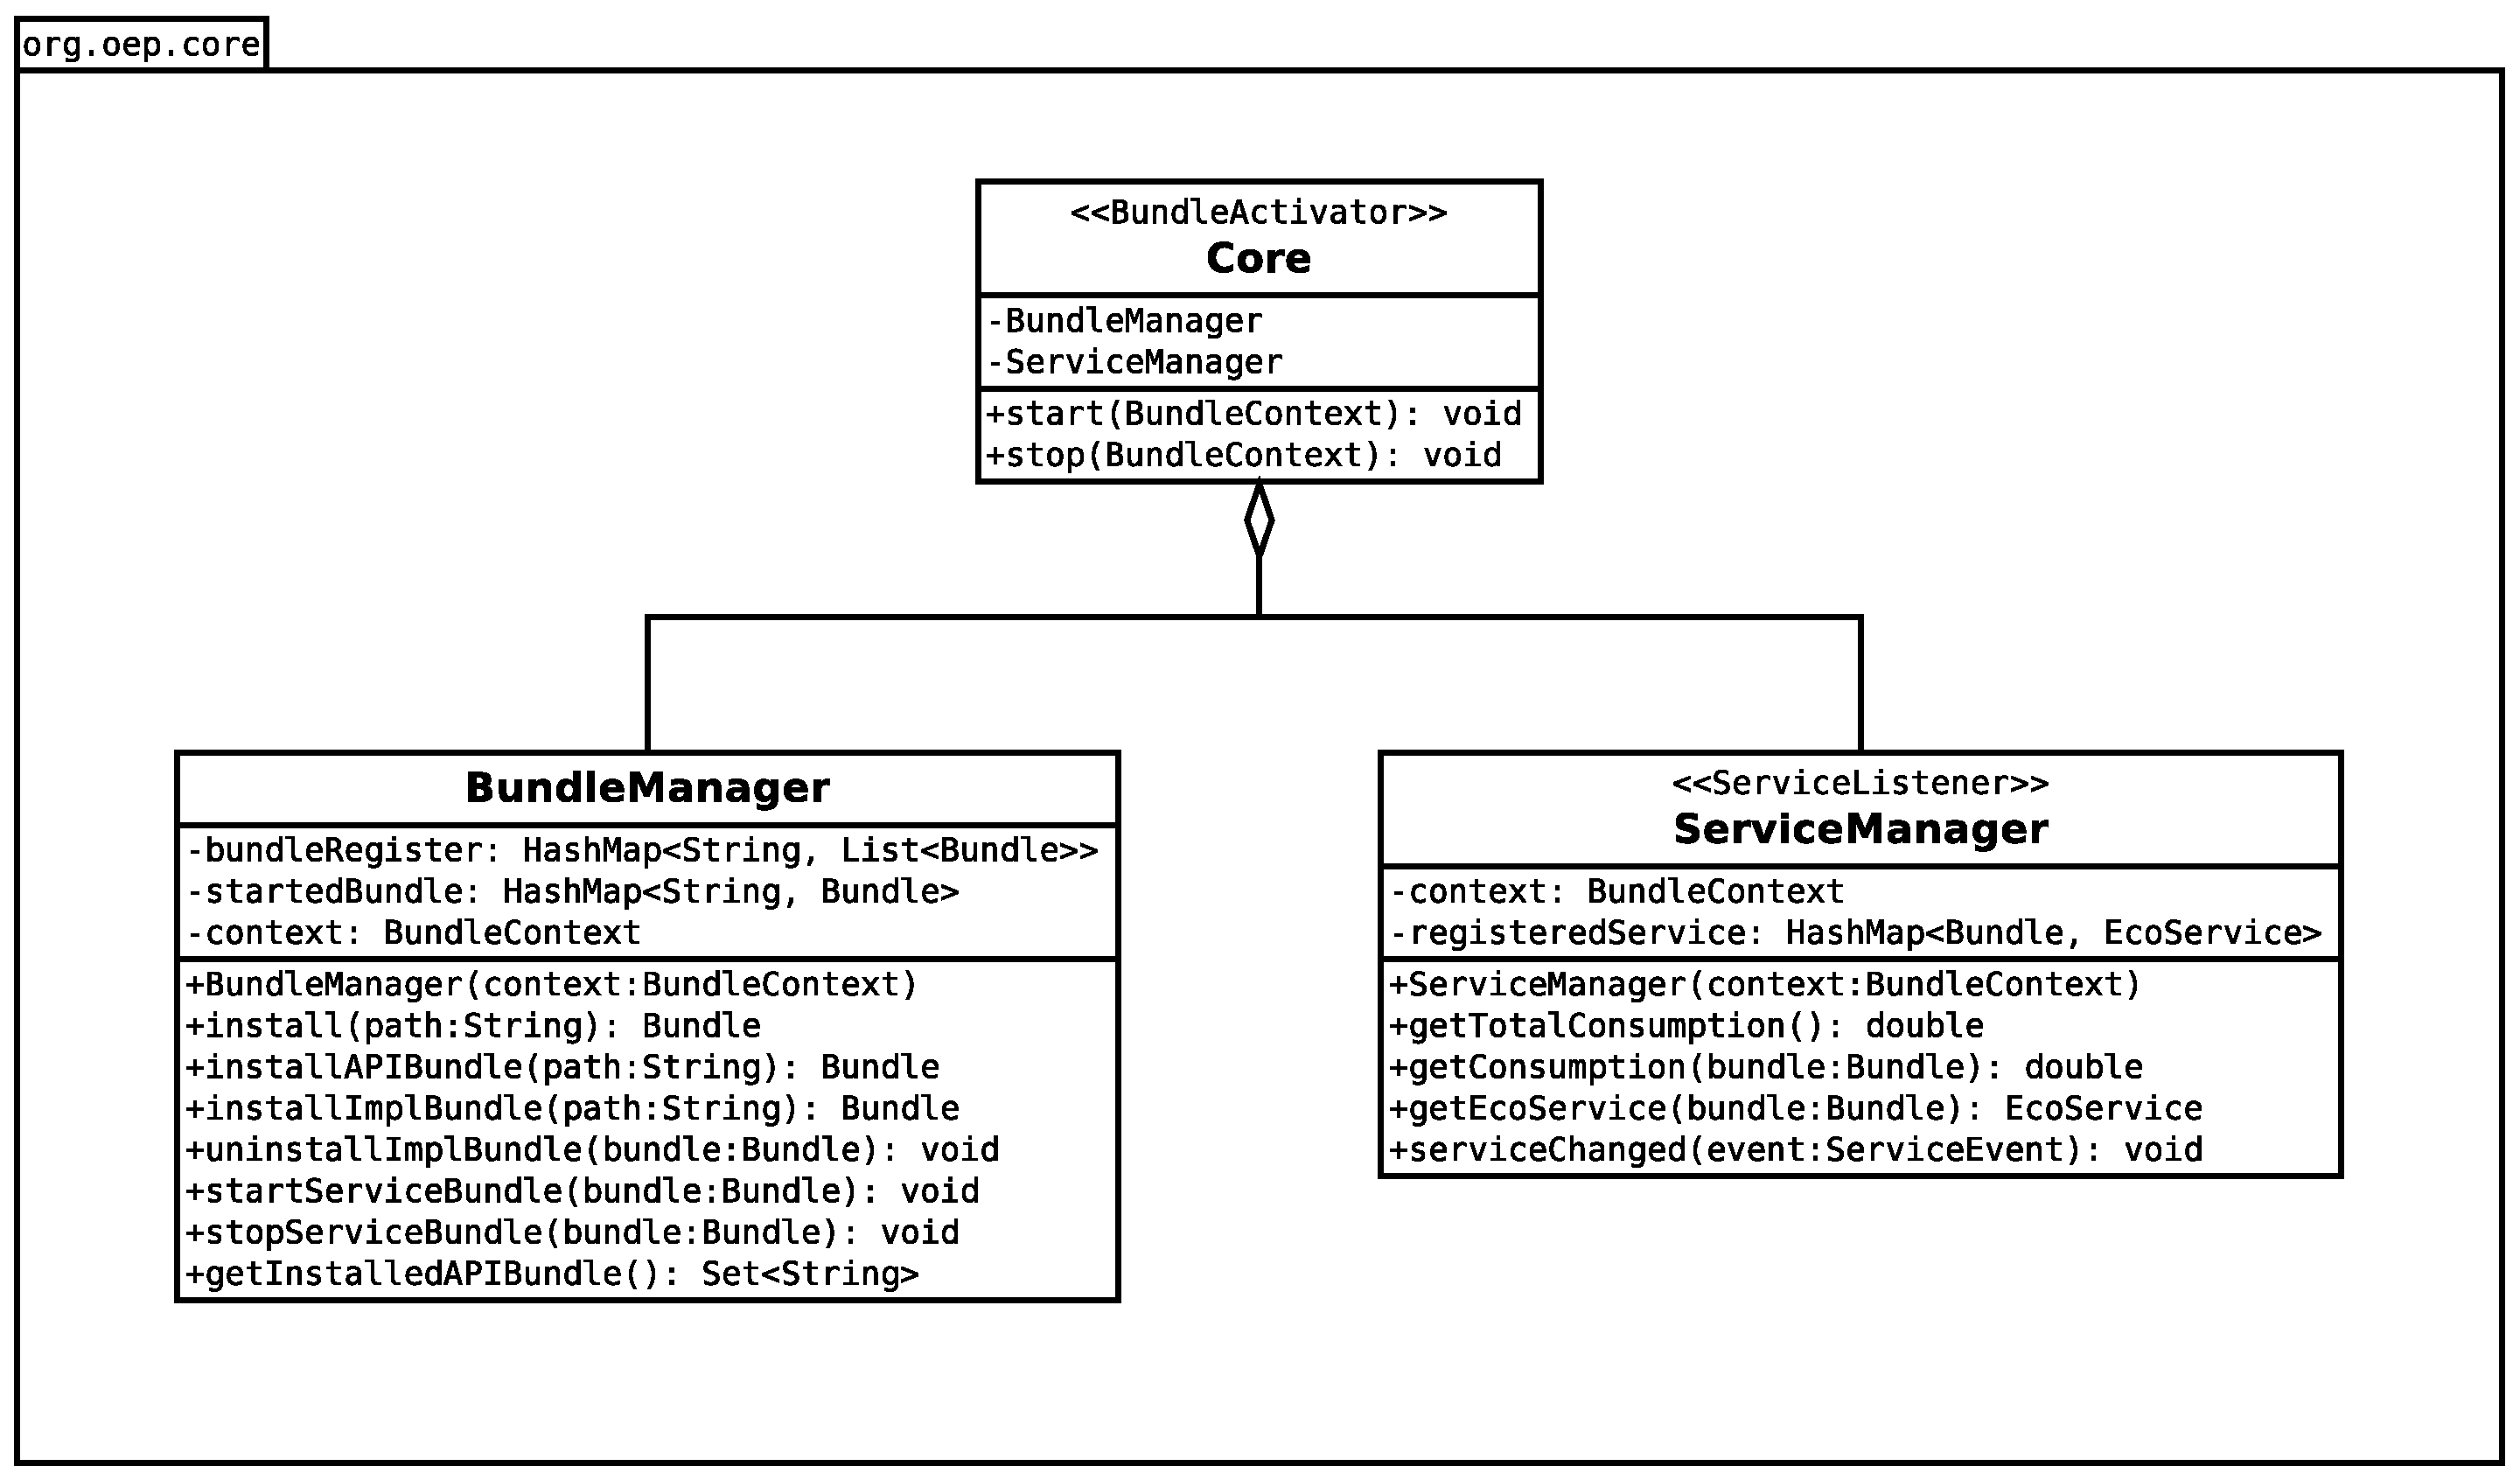
\includegraphics[width=0.99\textwidth]{figures/EcoPattern_Core_Classes.eps}
	\end{centering}
\section{Package org.oep.shell}
	\begin{centering}
		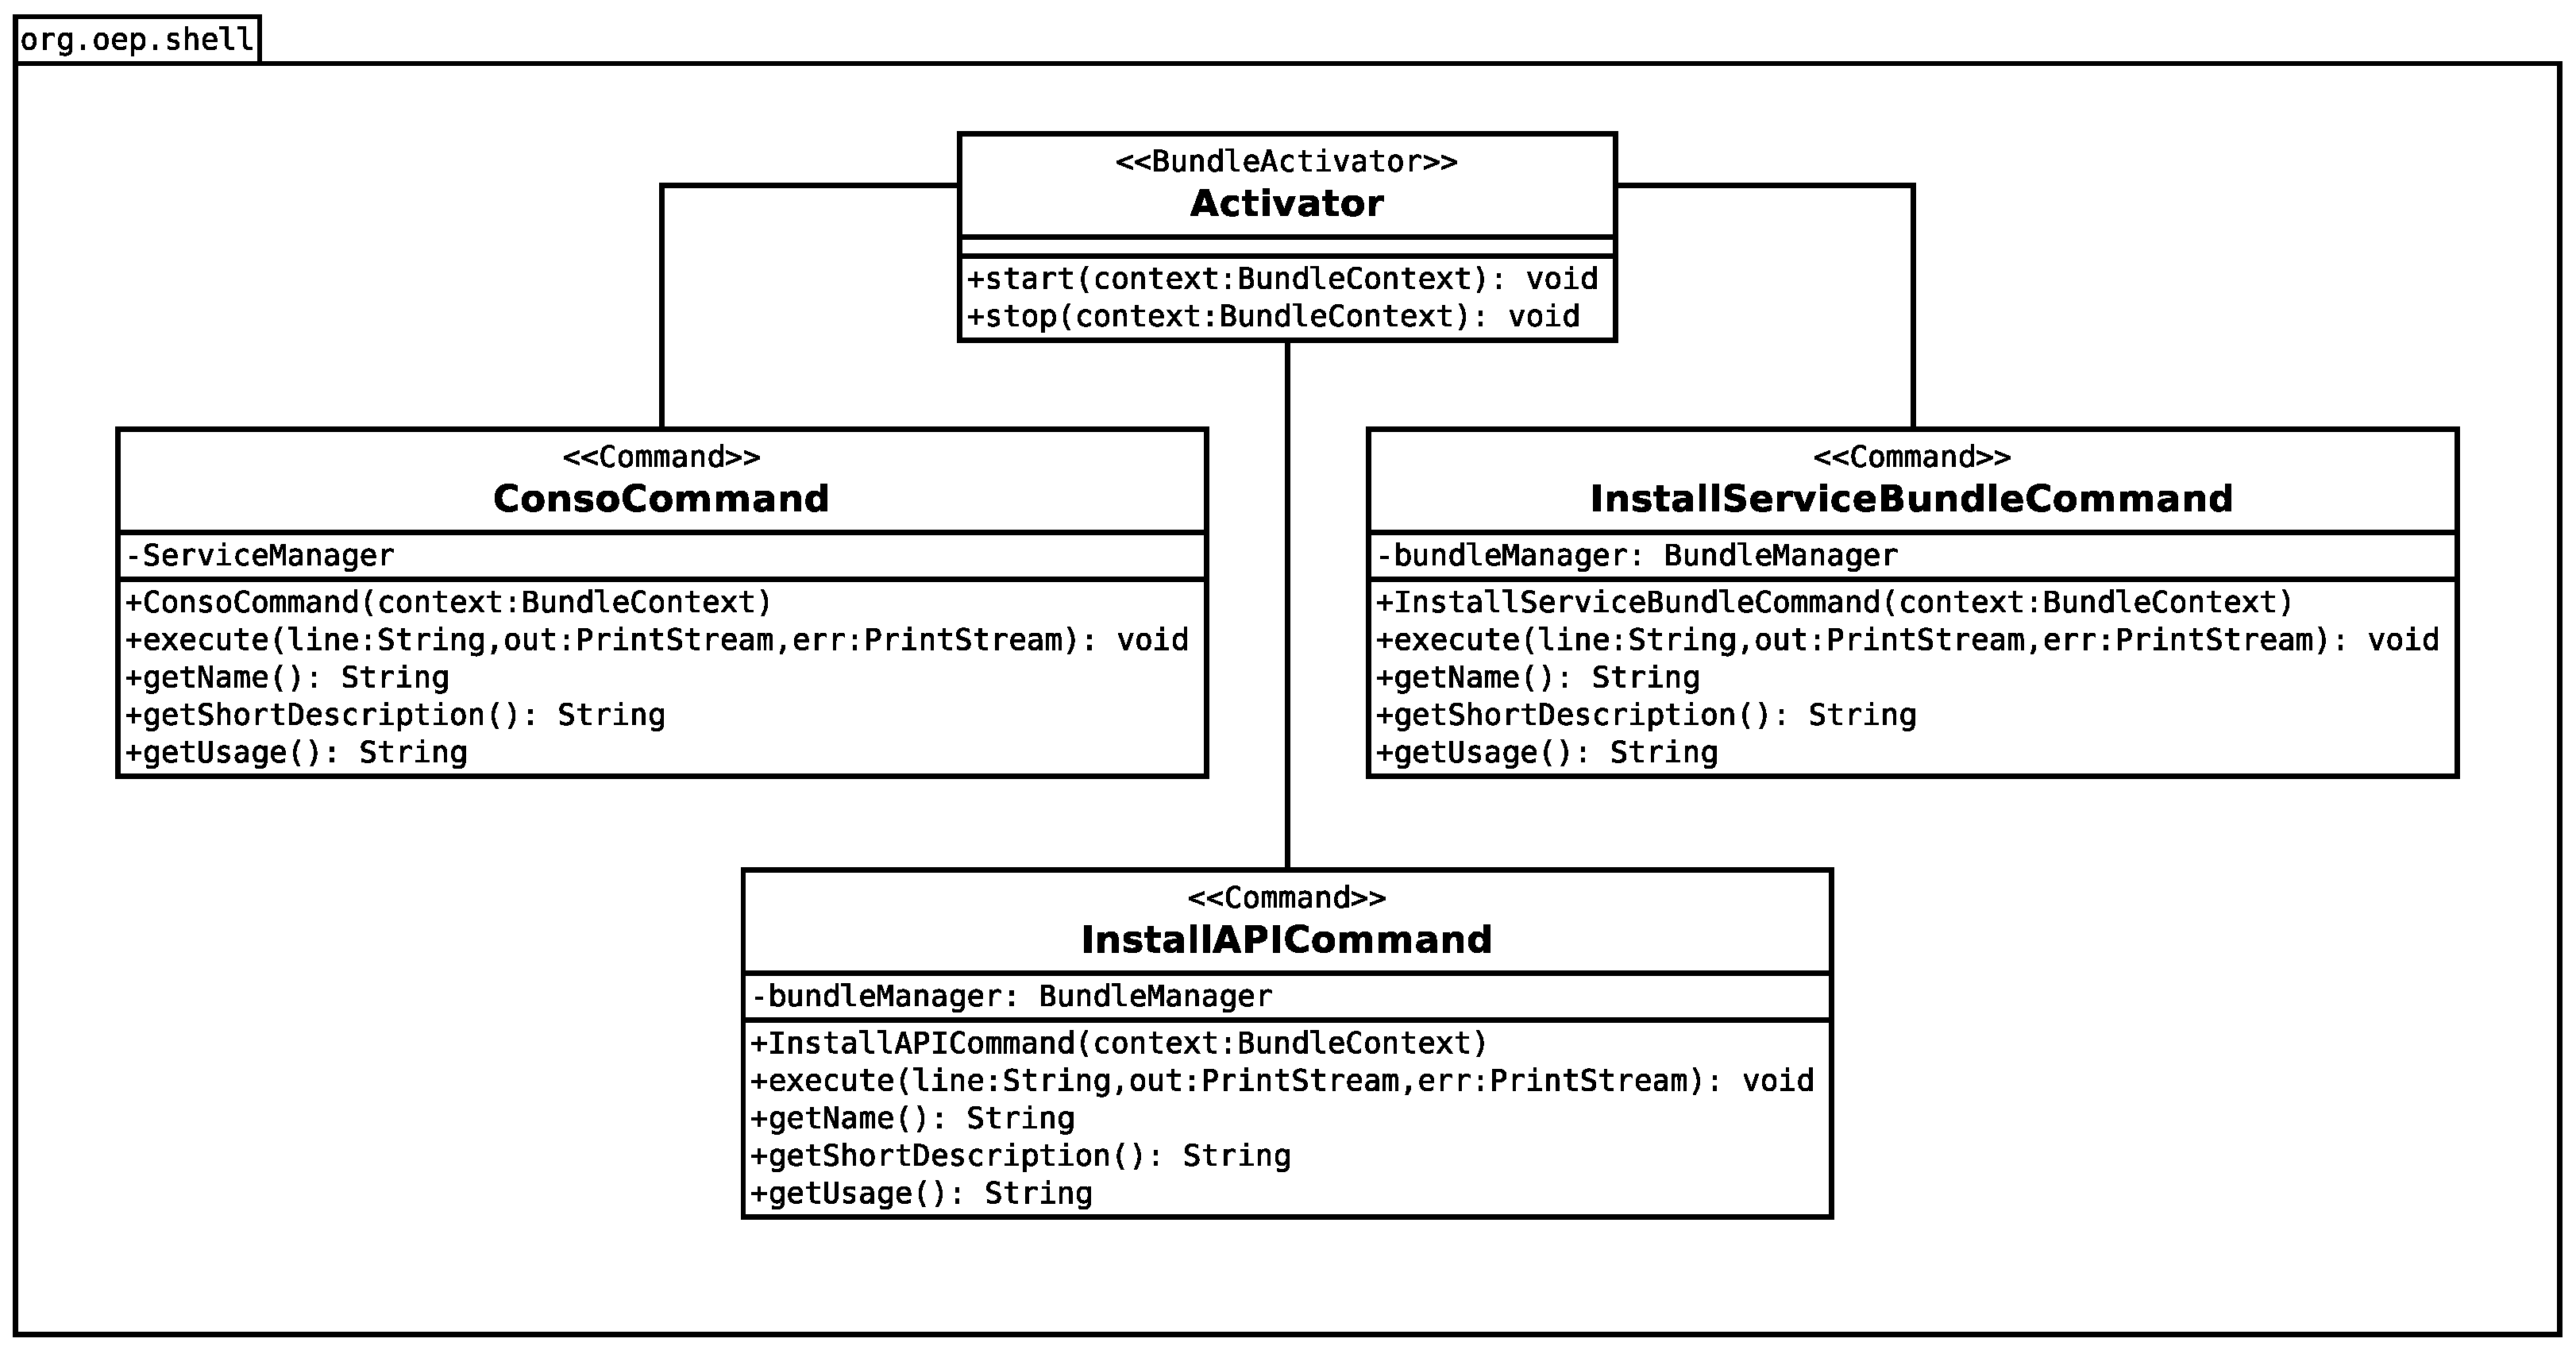
\includegraphics[width=0.99\textwidth]{figures/EcoPattern_Shell_Classes.eps}
	\end{centering}
\section{Package org.oep.gui}
	\begin{centering}
		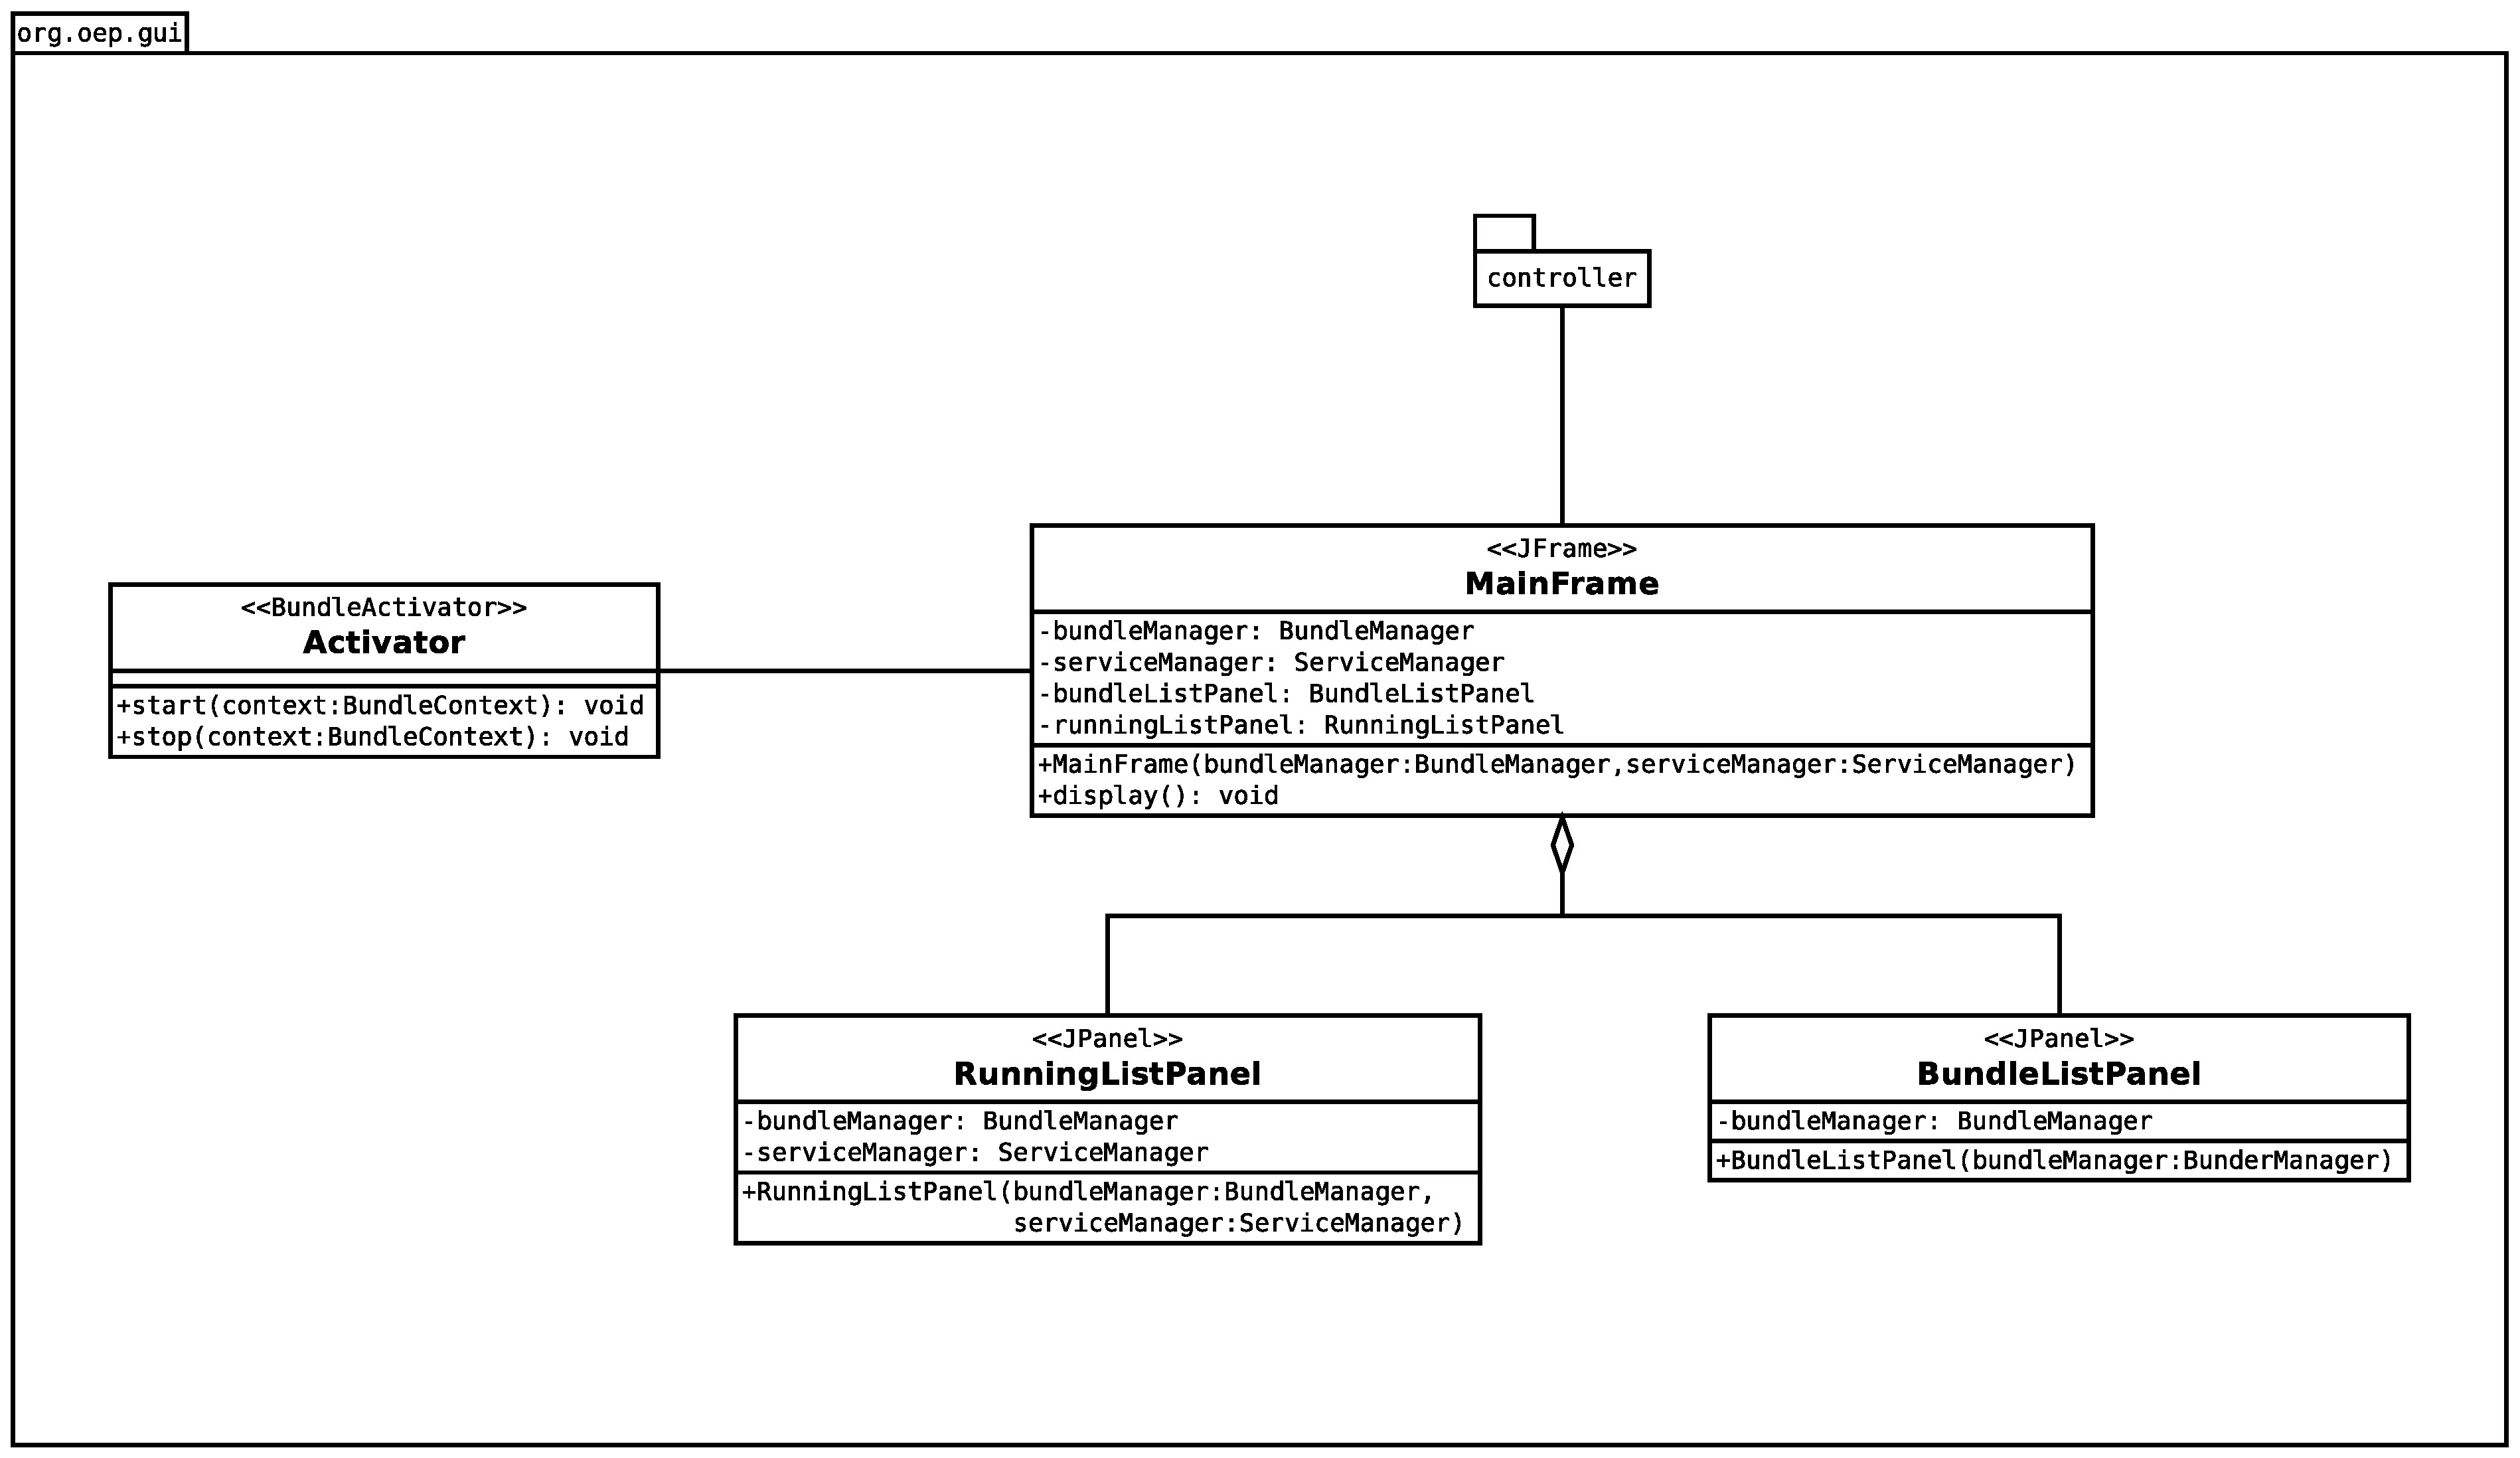
\includegraphics[width=0.99\textwidth]{figures/EcoPattern_Gui_Classes.eps}
	\end{centering}
\section{Package org.oep.core.controller.basic}
	\begin{centering}
		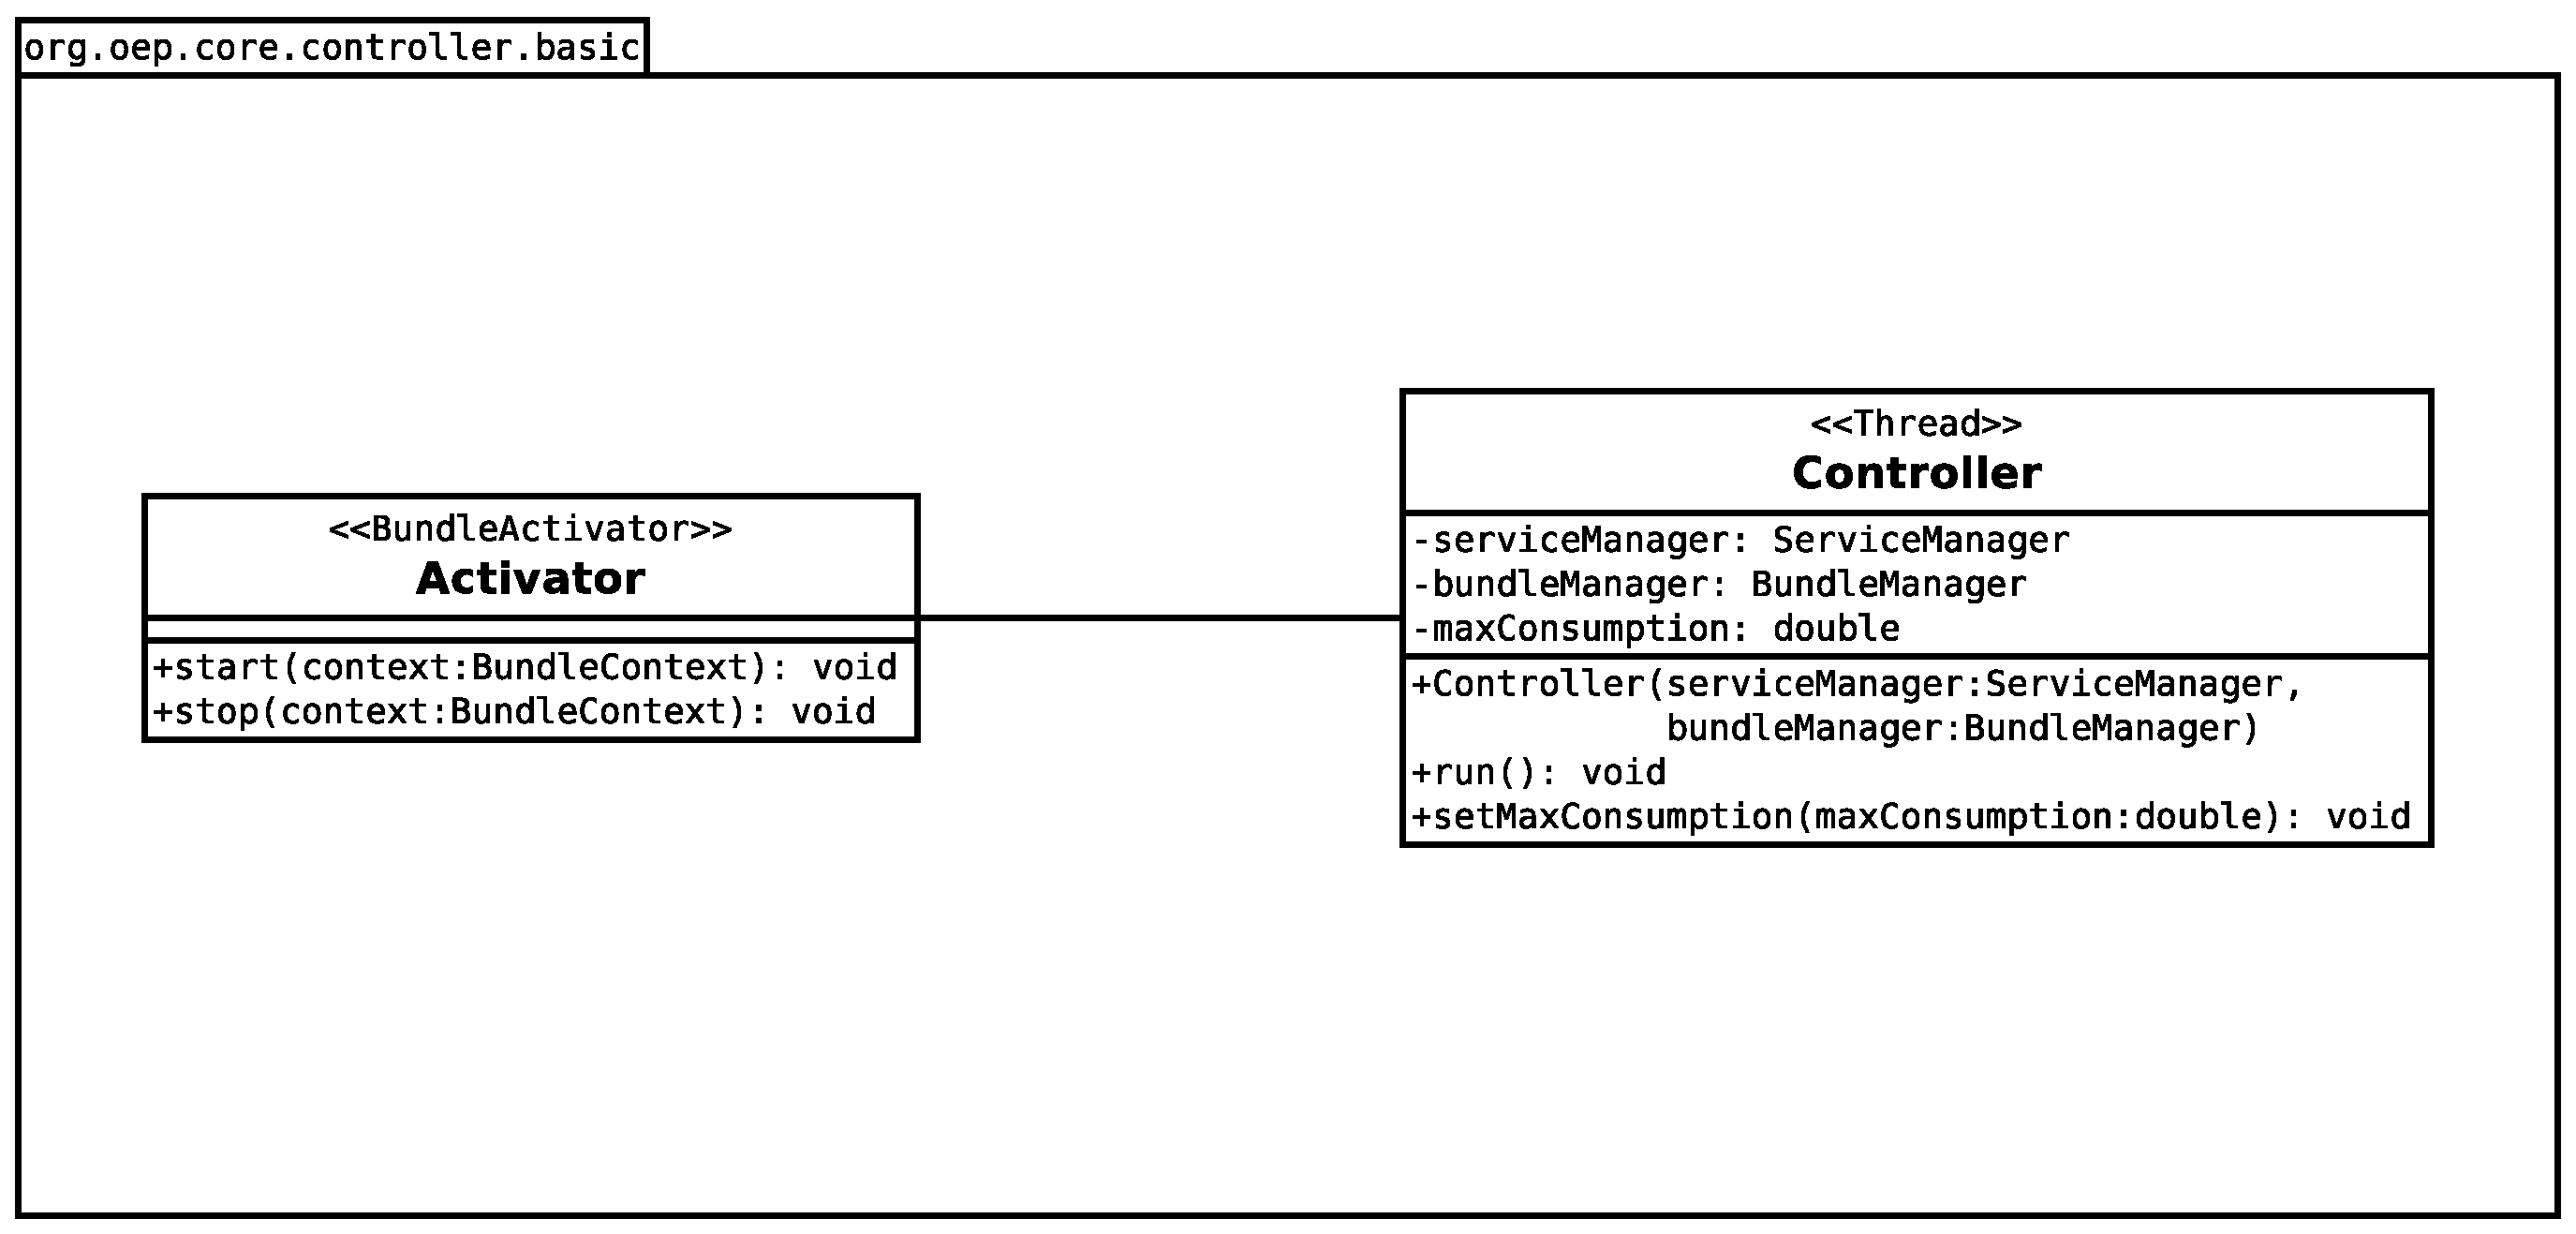
\includegraphics[width=0.99\textwidth]{figures/EcoPattern_Controller_Basic_Classes.eps}
	\end{centering}
\section{Package org.oep.service.api}
	\begin{centering}
		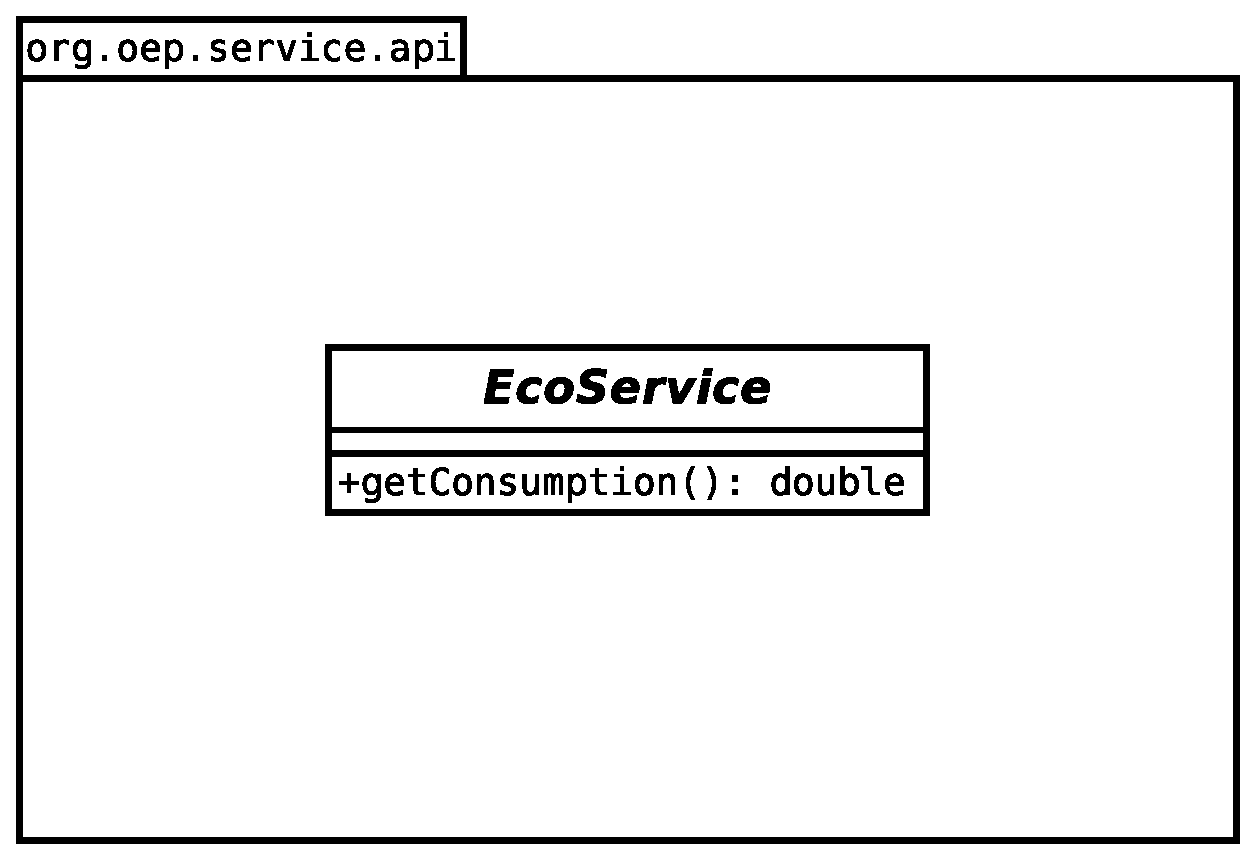
\includegraphics[width=0.45\textwidth]{figures/EcoPattern_Service_Api_Classes.eps}
	\end{centering}
\end{document}